% Options for packages loaded elsewhere
\PassOptionsToPackage{unicode}{hyperref}
\PassOptionsToPackage{hyphens}{url}
\PassOptionsToPackage{dvipsnames,svgnames,x11names}{xcolor}
%
\documentclass[
]{elegantbook}
\usepackage{amsmath,amssymb}
\usepackage{iftex}
\ifPDFTeX
  \usepackage[T1]{fontenc}
  \usepackage[utf8]{inputenc}
  \usepackage{textcomp} % provide euro and other symbols
\else % if luatex or xetex
  \ifXeTeX
    \usepackage{mathspec} % this also loads fontspec
  \else
    \usepackage{unicode-math} % this also loads fontspec
  \fi
  \defaultfontfeatures{Scale=MatchLowercase}
  \defaultfontfeatures[\rmfamily]{Ligatures=TeX,Scale=1}
\fi
\usepackage{lmodern}
\ifPDFTeX\else
  % xetex/luatex font selection
\fi
% Use upquote if available, for straight quotes in verbatim environments
\IfFileExists{upquote.sty}{\usepackage{upquote}}{}
\IfFileExists{microtype.sty}{% use microtype if available
  \usepackage[]{microtype}
  \UseMicrotypeSet[protrusion]{basicmath} % disable protrusion for tt fonts
}{}
\makeatletter
\@ifundefined{KOMAClassName}{% if non-KOMA class
  \IfFileExists{parskip.sty}{%
    \usepackage{parskip}
  }{% else
    \setlength{\parindent}{0pt}
    \setlength{\parskip}{6pt plus 2pt minus 1pt}}
}{% if KOMA class
  \KOMAoptions{parskip=half}}
\makeatother
\usepackage{xcolor}
\usepackage{color}
\usepackage{fancyvrb}
\newcommand{\VerbBar}{|}
\newcommand{\VERB}{\Verb[commandchars=\\\{\}]}
\DefineVerbatimEnvironment{Highlighting}{Verbatim}{commandchars=\\\{\}}
% Add ',fontsize=\small' for more characters per line
\usepackage{framed}
\definecolor{shadecolor}{RGB}{248,248,248}
\newenvironment{Shaded}{\begin{snugshade}}{\end{snugshade}}
\newcommand{\AlertTok}[1]{\textcolor[rgb]{0.94,0.16,0.16}{#1}}
\newcommand{\AnnotationTok}[1]{\textcolor[rgb]{0.56,0.35,0.01}{\textbf{\textit{#1}}}}
\newcommand{\AttributeTok}[1]{\textcolor[rgb]{0.13,0.29,0.53}{#1}}
\newcommand{\BaseNTok}[1]{\textcolor[rgb]{0.00,0.00,0.81}{#1}}
\newcommand{\BuiltInTok}[1]{#1}
\newcommand{\CharTok}[1]{\textcolor[rgb]{0.31,0.60,0.02}{#1}}
\newcommand{\CommentTok}[1]{\textcolor[rgb]{0.56,0.35,0.01}{\textit{#1}}}
\newcommand{\CommentVarTok}[1]{\textcolor[rgb]{0.56,0.35,0.01}{\textbf{\textit{#1}}}}
\newcommand{\ConstantTok}[1]{\textcolor[rgb]{0.56,0.35,0.01}{#1}}
\newcommand{\ControlFlowTok}[1]{\textcolor[rgb]{0.13,0.29,0.53}{\textbf{#1}}}
\newcommand{\DataTypeTok}[1]{\textcolor[rgb]{0.13,0.29,0.53}{#1}}
\newcommand{\DecValTok}[1]{\textcolor[rgb]{0.00,0.00,0.81}{#1}}
\newcommand{\DocumentationTok}[1]{\textcolor[rgb]{0.56,0.35,0.01}{\textbf{\textit{#1}}}}
\newcommand{\ErrorTok}[1]{\textcolor[rgb]{0.64,0.00,0.00}{\textbf{#1}}}
\newcommand{\ExtensionTok}[1]{#1}
\newcommand{\FloatTok}[1]{\textcolor[rgb]{0.00,0.00,0.81}{#1}}
\newcommand{\FunctionTok}[1]{\textcolor[rgb]{0.13,0.29,0.53}{\textbf{#1}}}
\newcommand{\ImportTok}[1]{#1}
\newcommand{\InformationTok}[1]{\textcolor[rgb]{0.56,0.35,0.01}{\textbf{\textit{#1}}}}
\newcommand{\KeywordTok}[1]{\textcolor[rgb]{0.13,0.29,0.53}{\textbf{#1}}}
\newcommand{\NormalTok}[1]{#1}
\newcommand{\OperatorTok}[1]{\textcolor[rgb]{0.81,0.36,0.00}{\textbf{#1}}}
\newcommand{\OtherTok}[1]{\textcolor[rgb]{0.56,0.35,0.01}{#1}}
\newcommand{\PreprocessorTok}[1]{\textcolor[rgb]{0.56,0.35,0.01}{\textit{#1}}}
\newcommand{\RegionMarkerTok}[1]{#1}
\newcommand{\SpecialCharTok}[1]{\textcolor[rgb]{0.81,0.36,0.00}{\textbf{#1}}}
\newcommand{\SpecialStringTok}[1]{\textcolor[rgb]{0.31,0.60,0.02}{#1}}
\newcommand{\StringTok}[1]{\textcolor[rgb]{0.31,0.60,0.02}{#1}}
\newcommand{\VariableTok}[1]{\textcolor[rgb]{0.00,0.00,0.00}{#1}}
\newcommand{\VerbatimStringTok}[1]{\textcolor[rgb]{0.31,0.60,0.02}{#1}}
\newcommand{\WarningTok}[1]{\textcolor[rgb]{0.56,0.35,0.01}{\textbf{\textit{#1}}}}
\usepackage{longtable,booktabs,array}
\usepackage{calc} % for calculating minipage widths
% Correct order of tables after \paragraph or \subparagraph
\usepackage{etoolbox}
\makeatletter
\patchcmd\longtable{\par}{\if@noskipsec\mbox{}\fi\par}{}{}
\makeatother
% Allow footnotes in longtable head/foot
\IfFileExists{footnotehyper.sty}{\usepackage{footnotehyper}}{\usepackage{footnote}}
\makesavenoteenv{longtable}
\usepackage{graphicx}
\makeatletter
\def\maxwidth{\ifdim\Gin@nat@width>\linewidth\linewidth\else\Gin@nat@width\fi}
\def\maxheight{\ifdim\Gin@nat@height>\textheight\textheight\else\Gin@nat@height\fi}
\makeatother
% Scale images if necessary, so that they will not overflow the page
% margins by default, and it is still possible to overwrite the defaults
% using explicit options in \includegraphics[width, height, ...]{}
\setkeys{Gin}{width=\maxwidth,height=\maxheight,keepaspectratio}
% Set default figure placement to htbp
\makeatletter
\def\fps@figure{htbp}
\makeatother
\setlength{\emergencystretch}{3em} % prevent overfull lines
\providecommand{\tightlist}{%
  \setlength{\itemsep}{0pt}\setlength{\parskip}{0pt}}
\setcounter{secnumdepth}{5}
\newlength{\cslhangindent}
\setlength{\cslhangindent}{1.5em}
\newlength{\csllabelwidth}
\setlength{\csllabelwidth}{3em}
\newlength{\cslentryspacingunit} % times entry-spacing
\setlength{\cslentryspacingunit}{\parskip}
\newenvironment{CSLReferences}[2] % #1 hanging-ident, #2 entry spacing
 {% don't indent paragraphs
  \setlength{\parindent}{0pt}
  % turn on hanging indent if param 1 is 1
  \ifodd #1
  \let\oldpar\par
  \def\par{\hangindent=\cslhangindent\oldpar}
  \fi
  % set entry spacing
  \setlength{\parskip}{#2\cslentryspacingunit}
 }%
 {}
\usepackage{calc}
\newcommand{\CSLBlock}[1]{#1\hfill\break}
\newcommand{\CSLLeftMargin}[1]{\parbox[t]{\csllabelwidth}{#1}}
\newcommand{\CSLRightInline}[1]{\parbox[t]{\linewidth - \csllabelwidth}{#1}\break}
\newcommand{\CSLIndent}[1]{\hspace{\cslhangindent}#1}
\definecolor{customcolor}{RGB}{32,178,170}
\colorlet{coverlinecolor}{customcolor}

% 下面如果不注释就准备好 Logo 和封面图片
% \logo{logo-blue.png} % 图片尺寸 1:1
% \cover{cover.jpg} % 图片尺寸 1280 × 1024

% Cancel common factors in Math 
\usepackage[makeroom]{cancel}

\usepackage[export]{adjustbox} %Needed for max width
%\patchcmd{<command>}{<code to replace>}{<code>}{<success>}{<failure>}
%The following codes add max dimension option to includegraphics
%Gin@ii is from graphicx package and looks for a second optional argument
\expandafter\patchcmd\csname Gin@ii\endcsname 
{\setkeys{Gin}{#1}}
{\setkeys{Gin}{max width=\textwidth, max height=.5\textwidth,keepaspectratio,#1}}
{}
{}

\definecolor{colortip}{RGB}{81,183,73}
\definecolor{colornote}{RGB}{251,188,5}
\definecolor{colorwarn}{RGB}{255,83,59}
\definecolor{colorinfo}{RGB}{204,204,204}

\tcbset{
  colbacktitle=white,
  enhanced,
  attach boxed title to top center={yshift=-2mm},
  colback=white, % 背景色
  coltext=black, % 文本色
  leftrule=1mm,
  rightrule=.25mm,
  bottomrule=.25mm,
  toprule=.25mm,
  boxsep=1pt, % 文字和边框的空隙
  arc=1pt % 圆角
}

\newtcolorbox{rmdtip}[1]{
  title=#1,
  coltitle=colortip,
  colframe=colortip, % 边框色
}

\newtcolorbox{rmdnote}[1]{
  title=#1,
  coltitle=colornote,
  colframe=colornote % 边框色
}

\newtcolorbox{rmdwarn}[1]{
  title=#1,
  coltitle=colorwarn,
  colframe=colorwarn % 边框色
}

\newtcolorbox{rmdinfo}{
  colframe=colorinfo % 边框色
}

\frontmatter
\usepackage[lotdepth=2, lofdepth=2]{subfig}
\usepackage[scale=0.85]{sourcecodepro}
\ifLuaTeX
  \usepackage{selnolig}  % disable illegal ligatures
\fi
\IfFileExists{bookmark.sty}{\usepackage{bookmark}}{\usepackage{hyperref}}
\IfFileExists{xurl.sty}{\usepackage{xurl}}{} % add URL line breaks if available
\urlstyle{same}
\hypersetup{
  pdftitle={Analisis Cluster dengan R},
  pdfauthor={Deden Istiawan},
  colorlinks=true,
  linkcolor={Maroon},
  filecolor={Maroon},
  citecolor={Blue},
  urlcolor={Blue},
  pdfcreator={LaTeX via pandoc}}

\title{Analisis Cluster dengan R}
\author{Deden Istiawan}
\date{}

\begin{document}
\maketitle

{
\hypersetup{linkcolor=}
\setcounter{tocdepth}{1}
\tableofcontents
}
\mainmatter

\begin{quote}
``Why is that when one man builds a wall, the next needs to to know what's on the other side?''

\hspace*{\fill} --- Tyrion Lannister-Game of Thrones
\end{quote}

\hypertarget{pengantar-analisis-cluster}{%
\chapter{Pengantar Analisis Cluster}\label{pengantar-analisis-cluster}}

\hypertarget{apa-itu-analisis-cluster}{%
\section{Apa itu Analisis Cluster?}\label{apa-itu-analisis-cluster}}

Analisis \emph{Cluster} mungkin salah satu yang paling banyak dipelajari dalam komunitas data mining dan \emph{machine learning} (\protect\hyperlink{ref-bandyopadhyay2011}{Bandyopadhyay, Saha, and Pedrycz 2011}). Masalah ini telah dipelajari oleh para peneliti dari berbagai disiplin ilmu selama lima dekade. Penerapan analisis \emph{cluster} mencakup berbagai domain masalah seperti teks, multimedia, jejaring sosial, dan data biologis. Clustering adalah topik yang agak beragam, dan algoritma yang mendasarinya sangat bergantung pada domain data dan skenario masalah (\protect\hyperlink{ref-2014clustering}{Aggarwal and Reddy 2014}). \emph{Clustering} adalah proses pengelompokan sekumpulan objek data menjadi beberapa kelompok atau \emph{cluster} sehingga objek yang berada di dalam \emph{cluster} memiliki kesamaan yang tinggi, tetapi sangat berbeda dengan objek di \emph{cluster} lain (\protect\hyperlink{ref-HanEtAl11}{Han, Kamber, and Pei 2011}). Pada buku ini akan dijelaskan konsep dasar dan metode analisis cluster, yang tediri dari: metode pengelompokan partisi dan hirarki, Model Probabilistik dan evaluasi algoritma \emph{clustering}.

Analisis \emph{cluster} atau \emph{clustering} adalah proses mengelompokkan sekumpulan objek data menjadi beberapa kelompok. Setiap subset adalah \emph{cluster}, sehingga objek dalam \emph{cluster} memiliki kemiripan yang sangat tinggi, namun berbeda dengan objek di \emph{cluster} lain. Himpunan \emph{cluster} yang dihasilkan dari analisis \emph{cluster} dapat disebut sebagai \emph{clustering}. Dalam konteks ini, algoritma \emph{clustering} yang berbeda dapat menghasilkan pengelompokan yang berbeda pada dataset yang sama. Oleh karena itu, pengelompokan berguna karena dapat mengarah pada penemuan kelompok yang sebelumnya tidak diketahui dalam data.

\hypertarget{apa-itu-bahasa-pemrograman-r}{%
\section{Apa itu Bahasa Pemrograman R?}\label{apa-itu-bahasa-pemrograman-r}}

R adalah bahasa pemrograman dan software bebas yang dikembangkan oleh Ross Ihaka dan Robert Gentleman pada tahun 1993. R memiliki katalog ekstensif metode statistik dan grafis. Ini meliputi algoritma machine learning, regresi linier, time series, inferensi statistik untuk beberapa hal. R tidak hanya diandalkan oleh para akademisi, tetapi juga banyak perusahaan besar menggunakan bahasa pemrograman R, antara lain Uber, Google, Airbnb, Facebook, dan masih banyak lagi.\footnote{\url{https://wartaekonomi.co.id/read375198/apa-itu-r-programming-language}}

\hypertarget{install-r-dan-rstudio}{%
\section{Install R dan RStudio}\label{install-r-dan-rstudio}}

Untuk menginstall R, kamu tidak memerlukan budget untuk membeli lisensi. R merupakan aplikasi open source sehingga dapat kamu unduh secara gratis di laman aslinya. Berikut langkah penginstallan mulai dari cara download hingga R siap digunakan. Pertama buka \href{https://cran.r-project.org/}{Halaman R Project}. Pilih installer sesuai sistem operasi. Misalnya pilih \textbf{Download R for Windows} dan pilih \textbf{install R for the first time}. Tunggu proses unduh instaler dan jika sudah 100\% terunduh klik file tersebut untuk mulai install R. setelah R berhasil diinstall langkah selanjutnya adalah menginstall program \href{https://posit.co/download/rstudio-desktop/}{RStudio}. Pada tahap ini kita akan install RStudio yaitu merupakan IDE yang umumnya digunakan untuk pemrograman R RStudio akan sangat membantu untuk melakukan coding R dan lainnya. Kita bisa langsung download installer versi terbaru atau jika ingin menggunakan versi sebelumnya bisa pilih all installer.

\hypertarget{menginstal-dan-memuat-r-packages}{%
\section{Menginstal dan memuat R packages}\label{menginstal-dan-memuat-r-packages}}

Setelah selesai instalI \href{https://cran.r-project.org/}{R} dan \href{https://posit.co/download/rstudio-desktop/}{RStudio}, serta memahami bagaimana menggunakannya, proses selanjutnya adalah instal R package. Kita dapat langsung melakukan instalasi R package yang sudah ada di \href{https://cran.r-project.org/}{CRAN} repository (mayoritas R package ada di sini) dengan menuliskan perintah \textbf{install.packages(``nama package'')} pada RStudio atau di Console. Kita harus terhubung dengan koneksi internet untuk dapat instal package. Misal, kita instal package \href{https://cran.r-project.org/web/packages/cluster/index.html}{\emph{cluster}}.

\begin{Shaded}
\begin{Highlighting}[]
\FunctionTok{install.packages}\NormalTok{(}\StringTok{"cluster"}\NormalTok{)}
\end{Highlighting}
\end{Shaded}

selain melalui \href{https://cran.r-project.org/}{CRAN} repository, intall packages juga dapat melaui \href{https://github.com/}{Github}. Anda harus terlebih dahulu harus menginstal \href{https://cran.r-project.org/web/packages/devtools/index.html}{devtools} jika Anda belum menginstalnya di komputer Anda. Misalnya, kode R berikut menginstal paket factoextra R versi terbaru yang dikembangkan oleh A. Kassambara (\url{https://github.com/kassambara/facoextra}) untuk analisis data multivariat dan visualisasi yang elegan.

\begin{Shaded}
\begin{Highlighting}[]
\FunctionTok{install.packages}\NormalTok{(}\StringTok{"devtools"}\NormalTok{)}
\NormalTok{devtools}\SpecialCharTok{::}\FunctionTok{install\_github}\NormalTok{(}\StringTok{"kassambara/factoextra"}\NormalTok{)}
\end{Highlighting}
\end{Shaded}

\begin{rmdnote}{Note}
Note that, GitHub contains the developmental version of R packages

\end{rmdnote}

Setelah instalasi, pertama-tama Anda harus memuat paket untuk menggunakan fungsi-fungsi di dalam paket. Fungsi \textbf{library()}.

\begin{Shaded}
\begin{Highlighting}[]
\FunctionTok{library}\NormalTok{(cluster)}
\end{Highlighting}
\end{Shaded}

\begin{lemma}
\protect\hypertarget{lem:chf-pdf}{}\label{lem:chf-pdf}For any two random variables \(X_1\), \(X_2\), they both have the same probability distribution if and only if \[\varphi _{X_1}(t)=\varphi _{X_2}(t)\]
\end{lemma}

\begin{theorem}
\protect\hypertarget{thm:chf-sum}{}\label{thm:chf-sum}If \(X_1\), \ldots, \(X_n\) are independent random variables, and \(a_1\), \ldots, \(a_n\) are some constants, then the characteristic function of the linear combination \(S_n=\sum_{i=1}^na_iX_i\) is \[\varphi _{S_{n}}(t)=\prod_{i=1}^n\varphi _{X_i}(a_{i}t)=\varphi _{X_{1}}(a_{1}t)\cdots \varphi _{X_{n}}(a_{n}t)\]
\end{theorem}

\begin{proposition}
\protect\hypertarget{prp:unnamed-chunk-4}{}\label{prp:unnamed-chunk-4}The distribution of the sum of independent Poisson random variables \(X_i \sim \mathrm{Pois}(\lambda_i),\: i=1,2,\cdots,n\) is \(\mathrm{Pois}(\sum_{i=1}^n\lambda_i)\).
\end{proposition}

\hypertarget{math-formular}{%
\section{Lorem Ipsum5}\label{math-formular}}

Lorem ipsum dolor sit amet, consectetur adipiscing elit, sed do eiusmod tempor incididunt ut labore et dolore magna aliqua. Ut enim ad minim veniam, quis nostrud exercitation ullamco laboris nisi ut aliquip ex ea commodo consequat. Duis aute irure dolor in reprehenderit in voluptate velit esse cillum dolore eu fugiat nulla pariatur. Excepteur sint occaecat cupidatat non proident, sunt in culpa qui officia deserunt mollit anim id est laborum. \footnote{\url{https://github.com/ElegantLaTeX/ElegantBook/blob/6ab10beda81252f0b478e05fa926199301347e4a/elegantbook.cls\#L884}}.

\begin{Shaded}
\begin{Highlighting}[]
\KeywordTok{\textless{}script}\OtherTok{ type=}\StringTok{"text/x{-}mathjax{-}config"}\KeywordTok{\textgreater{}}
\NormalTok{    MathJax}\OperatorTok{.}\AttributeTok{Hub}\OperatorTok{.}\FunctionTok{Config}\NormalTok{(\{}
      \DataTypeTok{TeX}\OperatorTok{:}\NormalTok{ \{}
        \DataTypeTok{Macros}\OperatorTok{:}\NormalTok{ \{}
          \DataTypeTok{bm}\OperatorTok{:}\NormalTok{ [}\StringTok{"\{}\SpecialCharTok{\textbackslash{}\textbackslash{}}\StringTok{boldsymbol \#1\}"}\OperatorTok{,}\DecValTok{1}\NormalTok{]}\OperatorTok{,}
\NormalTok{        \}}
\NormalTok{      \}}
\NormalTok{    \})}\OperatorTok{;}
\KeywordTok{\textless{}/script\textgreater{}}
\end{Highlighting}
\end{Shaded}

Lorem ipsum dolor sit amet, consectetur adipiscing elit, sed do eiusmod tempor incididunt ut labore et dolore magna aliqua. Ut enim ad minim veniam, quis nostrud exercitation ullamco laboris nisi ut aliquip ex ea commodo consequat. Duis aute irure dolor in reprehenderit in voluptate velit esse cillum dolore eu fugiat nulla pariatur. Excepteur sint occaecat cupidatat non proident, sunt in culpa qui officia deserunt mollit anim id est laborum.

\begin{Shaded}
\begin{Highlighting}[]
\KeywordTok{\textless{}script}\OtherTok{ type=}\StringTok{"text/x{-}mathjax{-}config"}\KeywordTok{\textgreater{}}
\NormalTok{    MathJax}\OperatorTok{.}\AttributeTok{Hub}\OperatorTok{.}\FunctionTok{Config}\NormalTok{(\{}
      \DataTypeTok{TeX}\OperatorTok{:}\NormalTok{ \{}
        \DataTypeTok{Macros}\OperatorTok{:}\NormalTok{ \{}
          \DataTypeTok{bm}\OperatorTok{:}\NormalTok{ [}\StringTok{"\{}\SpecialCharTok{\textbackslash{}\textbackslash{}}\StringTok{boldsymbol \#1\}"}\OperatorTok{,}\DecValTok{1}\NormalTok{]}\OperatorTok{,}
\NormalTok{        \}}\OperatorTok{,}
        \DataTypeTok{extensions}\OperatorTok{:}\NormalTok{ [}\StringTok{"cancel.js"}\NormalTok{]}
\NormalTok{      \}}
\NormalTok{    \})}\OperatorTok{;}
\KeywordTok{\textless{}/script\textgreater{}}
\end{Highlighting}
\end{Shaded}

Lorem ipsum dolor sit amet, consectetur adipiscing elit, sed do eiusmod tempor incididunt ut labore et dolore magna aliqua. Ut enim ad minim veniam, quis nostrud exercitation ullamco laboris nisi ut aliquip ex ea commodo consequat. Duis aute irure dolor in reprehenderit in voluptate velit esse cillum dolore eu fugiat nulla pariatur. Excepteur sint occaecat cupidatat non proident, sunt in culpa qui officia deserunt mollit anim id est laborum.

\begin{Shaded}
\begin{Highlighting}[]
\BuiltInTok{\textbackslash{}usepackage}\NormalTok{[makeroom]\{}\ExtensionTok{cancel}\NormalTok{\}}
\end{Highlighting}
\end{Shaded}

\hypertarget{custom-block}{%
\section{Lorem Ipsum6}\label{custom-block}}

Lorem ipsum dolor sit amet, consectetur adipiscing elit, sed do eiusmod tempor incididunt ut labore et dolore magna aliqua. Ut enim ad minim veniam, quis nostrud exercitation ullamco laboris nisi ut aliquip ex ea commodo consequat. Duis aute irure dolor in reprehenderit in voluptate velit esse cillum dolore eu fugiat nulla pariatur. Excepteur sint occaecat cupidatat non proident, sunt in culpa qui officia deserunt mollit anim id est laborum. \url{https://bookdown.org/yihui/rmarkdown-cookbook/custom-blocks.html}.

\textcolor{red}{\textbf{TODO: }{there is still a lot to do}}

\begin{rmdwarn}{Warning}
Warning

\end{rmdwarn}

\begin{rmdtip}{Tips}
Tips

\end{rmdtip}

\begin{rmdnote}{Note}
Note

\end{rmdnote}

Info

\hypertarget{algoritma-k-means}{%
\chapter{Algoritma K-Means}\label{algoritma-k-means}}

\hypertarget{pengantar-algoritam-k-means}{%
\section{Pengantar Algoritam K-Means}\label{pengantar-algoritam-k-means}}

K-means merupakan salah satu metode hard partition yang banyak digunakan untuk pengelompokan data. Algoritma K-means adalah dasar pengelompokan metode partisi yang dipublikasikan oleh Lloyd dari Bell Telephone Laboratories pada tahun 1957. Penelitian pada K-means dapat ditelusuri kembali ke pertengahan abad yang lalu, yang dilakukan oleh berbagai peneliti diseluruh disiplin ilmu yang berbeda terutama oleh Lloyd (1957), Forgey (1965), Friedman dan Robin (1967) dan MacQueen (1967). K-means dapat didefinisikan sebagai algoritma klastering yang mengelompokan data ke dalam k klaster berdasarkan jarak terdekat data dengan pusat klaster. Algoritma K-means sangat efisien untuk mengelompokan dataset yang besar, kemudahan dalam pengaplikasiannya dan metode yang efisien dalam hal komputasi, menjadi alasan utama popularitas K-means, meskipun telah diusulkan lebih dari 50 tahun yang lalu.

Algoritma K-means mengelompokan objek ke dalam kelompok sehingga objek dalam satu klaster memiliki kemiripan yang tinggi dibandingkan dengan objek di dalam klaster yang berbeda. K-means dimulai dengan menentukan jumlah klaster sebanyak k, kemudian membangkitkan k pusat klaster secara acak. Selanjutnya setiap objek akan dikelompokan berdasarkan jarak terdekat dengan pusat klaster, pusat klaster diperbaharui berdasarkan titik data dalam setiap klaster. Proses ini diulangi sampai kriteria konvergen terpenuhi. Berikut ini adalah tahapan dari algoritma K-means:

\begin{enumerate}
\def\labelenumi{\arabic{enumi}.}
\item
  Menentukan nilai k sebagai jumlah klaster yang dibentuk.
\item
  Memilih k pusat klaster secara acak untuk menjadi pusat klaster awal.
\item
  Alokasikan semua data ke pusat klaster terdekat dengan matrik jarak.
\item
  Hitung kembali pusat klaster baru berdasarkan data yang mengikuti klaster masing-masing.
\item
  Ulangi langkah 3 dan 4 hingga kondisi konvergen tercapai atau tidak ada data yang berpindah dari satu klaster ke klaster yang lainnya.
\end{enumerate}

\hypertarget{eksperimen-algoritma-k-means}{%
\section{Eksperimen Algoritma K-Means}\label{eksperimen-algoritma-k-means}}

Pada eksprimen ini algoritma K-Means akan digunakan untuk mengelompokan data kemiskinan di Jawa Tengah yang diambil dari website Tim Percepatan Penanggulangan Kemiskinan \href{https://www.tnp2k.go.id/}{(TNP2K)}

\hypertarget{data}{%
\subsection{Data}\label{data}}

Package \texttt{reader} menyiapkan fungsi \href{https://readr.tidyverse.org/reference/read_delim.html}{\texttt{read\_csv()}} untuk import data dari file CSV. Pada kasus ini digunakan data \href{https://github.com/dedenistiawan/Dataset/blob/main/BDT.csv}{Data 40\% Kemiskinan di jawa Tengah}.

\begin{Shaded}
\begin{Highlighting}[]
\FunctionTok{library}\NormalTok{ (readr)}
\NormalTok{urlfile }\OtherTok{=} \StringTok{"https://raw.githubusercontent.com/dedenistiawan/Dataset/main/Basis\%20Data\%20Terpadu\%20Jateng.csv"}

\NormalTok{data}\OtherTok{\textless{}{-}}\FunctionTok{read.csv}\NormalTok{(}\FunctionTok{url}\NormalTok{(urlfile), }\AttributeTok{row.names =} \StringTok{"Kabupaten"}\NormalTok{)}
\end{Highlighting}
\end{Shaded}

\begin{Shaded}
\begin{Highlighting}[]
\NormalTok{knitr}\SpecialCharTok{::}\FunctionTok{kable}\NormalTok{(}
  \FunctionTok{head}\NormalTok{(data, }\DecValTok{10}\NormalTok{), }\AttributeTok{caption =} \StringTok{\textquotesingle{}Basis Data Terpadu Jawa Tengah\textquotesingle{}}\NormalTok{,}
  \AttributeTok{booktabs =} \ConstantTok{TRUE}\NormalTok{)}
\end{Highlighting}
\end{Shaded}

\begin{longtable}[]{@{}lrrrrrrrrrr@{}}
\caption{\label{tab:nice-tab}Basis Data Terpadu Jawa Tengah}\tabularnewline
\toprule\noalign{}
& X1 & X2 & X3 & X4 & X5 & X6 & X7 & X8 & X9 & X10 \\
\midrule\noalign{}
\endfirsthead
\toprule\noalign{}
& X1 & X2 & X3 & X4 & X5 & X6 & X7 & X8 & X9 & X10 \\
\midrule\noalign{}
\endhead
\bottomrule\noalign{}
\endlastfoot
CILACAP & 5.19 & 5.67 & 5.08 & 5.44 & 5.22 & 6.05 & 11.47 & 9.78 & 5.55 & 5.12 \\
BANYUMAS & 5.71 & 4.47 & 5.18 & 5.51 & 5.02 & 6.21 & 7.39 & 6.96 & 5.98 & 8.22 \\
PURBALINGGA & 3.30 & 2.19 & 3.80 & 3.13 & 3.73 & 3.34 & 8.71 & 7.41 & 3.21 & 4.65 \\
BANJARNEGARA & 2.73 & 2.34 & 3.76 & 2.80 & 2.57 & 2.99 & 3.31 & 5.45 & 4.21 & 6.05 \\
KEBUMEN & 4.17 & 2.55 & 3.26 & 4.16 & 3.15 & 4.15 & 4.30 & 9.29 & 4.61 & 4.34 \\
PURWOREJO & 1.87 & 2.12 & 1.48 & 3.05 & 1.78 & 1.83 & 5.00 & 4.90 & 3.12 & 2.09 \\
WONOSOBO & 2.13 & 1.95 & 3.00 & 1.78 & 1.62 & 2.06 & 0.45 & 2.32 & 3.57 & 0.84 \\
MAGELANG & 3.95 & 3.01 & 4.22 & 4.15 & 3.01 & 3.64 & 1.44 & 3.35 & 5.69 & 3.67 \\
BOYOLALI & 2.19 & 3.07 & 1.61 & 2.74 & 2.11 & 1.82 & 1.71 & 2.34 & 3.41 & 1.55 \\
KLATEN & 3.84 & 5.15 & 1.93 & 4.64 & 4.04 & 3.78 & 8.71 & 4.45 & 3.99 & 3.09 \\
\end{longtable}

\hypertarget{memeriksa-missing-value}{%
\subsection{Memeriksa Missing Value}\label{memeriksa-missing-value}}

\begin{Shaded}
\begin{Highlighting}[]
\FunctionTok{colSums}\NormalTok{(}\FunctionTok{is.na}\NormalTok{(data))}
\end{Highlighting}
\end{Shaded}

\begin{verbatim}
##  X1  X2  X3  X4  X5  X6  X7  X8  X9 X10 
##   0   0   0   0   0   0   0   0   0   0
\end{verbatim}

Hasil output di atas menunjukan bahwa tidak \emph{missing value} di semua variabel

\hypertarget{visualisasi-matriks-jarak}{%
\subsection{Visualisasi Matriks jarak}\label{visualisasi-matriks-jarak}}

\begin{Shaded}
\begin{Highlighting}[]
\CommentTok{\#Plot Disatance}
\FunctionTok{library}\NormalTok{(ggplot2)}
\FunctionTok{library}\NormalTok{(factoextra)}
\NormalTok{distance }\OtherTok{\textless{}{-}} \FunctionTok{get\_dist}\NormalTok{(data)}
\FunctionTok{fviz\_dist}\NormalTok{(distance, }\AttributeTok{gradient =} \FunctionTok{list}\NormalTok{(}\AttributeTok{low =} \StringTok{"\#00AFBB"}\NormalTok{, }\AttributeTok{mid =} \StringTok{"white"}\NormalTok{, }\AttributeTok{high =} \StringTok{"\#FC4E07"}\NormalTok{))}
\end{Highlighting}
\end{Shaded}

\begin{figure}

{\centering 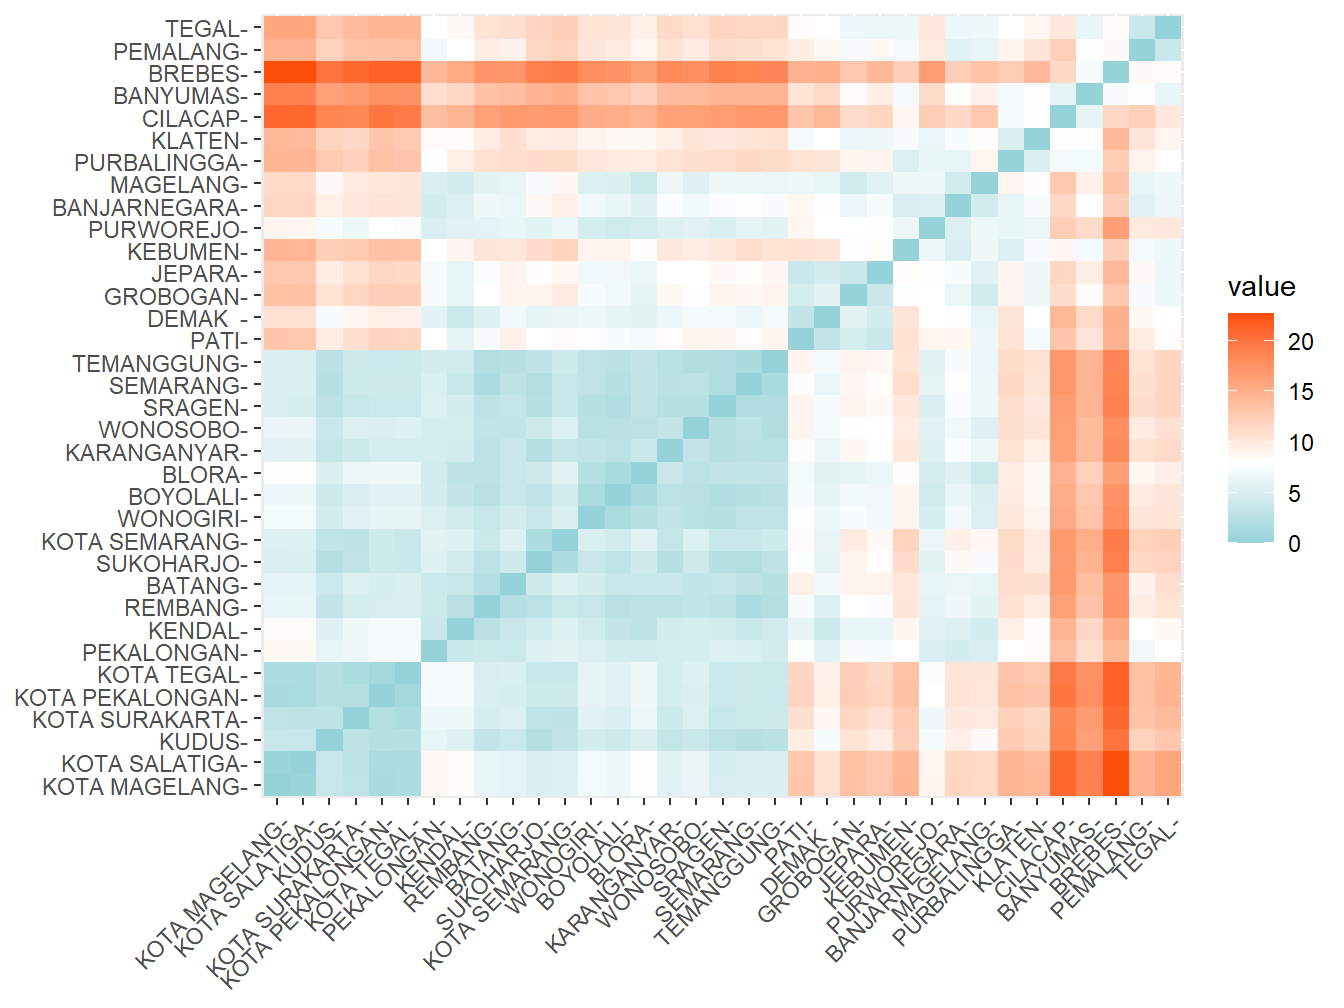
\includegraphics[width=0.8\linewidth]{01-KM_files/figure-latex/unnamed-chunk-2-1} 

}

\caption{Matrik Jarak}\label{fig:unnamed-chunk-2}
\end{figure}

Matriks jarak ini berfungsi untuk mengukur jarak antar variabel, semakin merah warnanya maka semakin jauh jarak antar variabel dan semakin biru semakin dekat jarak antar variabel.

\hypertarget{estimasi-jumlah-cluster-optimal}{%
\subsection{\texorpdfstring{Estimasi Jumlah \emph{Cluster} Optimal}{Estimasi Jumlah Cluster Optimal}}\label{estimasi-jumlah-cluster-optimal}}

Dalam metode k-means banyaknya klaster ditentukan sendiri oleh pengguna. Maka dari itu perlu dicari jumlah klaster yang optimum yang dapat mengelompokkan objek dengan baik (Perlu diketahui bahwa metode ini relatif subjektif). Salah satu metode yang digunakan adalah Elbow Plot. Elbow Plot merupakan plot antara banyak klaster dengan total within-cluster variation (total dari simpangan per kluster). Banyak klaster yang dipilih adalah bagian ``siku'' atau titik dimana terdapat penurunan yang tajam sebelum titik tersebut dan disusul penurunan yang tidak tajam setelah titik tersebut. Hal ini karena penambahan jumlah klaster tidak membawa pengaruh banyak atas variasi yang ada di dalam klaster tersebut.

\hypertarget{membuat-plot-cluster}{%
\subsection{\texorpdfstring{Membuat Plot \emph{Cluster}}{Membuat Plot Cluster}}\label{membuat-plot-cluster}}

Jumlah klaster yang dibentuk mulai dari 2 sampai 5, untuk melihat sebaran data pada masing-masing \emph{cluster}

\begin{Shaded}
\begin{Highlighting}[]
\CommentTok{\#use several different values of k}
\NormalTok{k2 }\OtherTok{\textless{}{-}} \FunctionTok{kmeans}\NormalTok{(data, }\AttributeTok{centers =} \DecValTok{2}\NormalTok{, }\AttributeTok{nstart =} \DecValTok{25}\NormalTok{)}
\NormalTok{k3 }\OtherTok{\textless{}{-}} \FunctionTok{kmeans}\NormalTok{(data, }\AttributeTok{centers =} \DecValTok{3}\NormalTok{, }\AttributeTok{nstart =} \DecValTok{25}\NormalTok{)}
\NormalTok{k4 }\OtherTok{\textless{}{-}} \FunctionTok{kmeans}\NormalTok{(data, }\AttributeTok{centers =} \DecValTok{4}\NormalTok{, }\AttributeTok{nstart =} \DecValTok{25}\NormalTok{)}
\NormalTok{k5 }\OtherTok{\textless{}{-}} \FunctionTok{kmeans}\NormalTok{(data, }\AttributeTok{centers =} \DecValTok{5}\NormalTok{, }\AttributeTok{nstart =} \DecValTok{25}\NormalTok{)}
\end{Highlighting}
\end{Shaded}

\begin{Shaded}
\begin{Highlighting}[]
\CommentTok{\# plots to compare}
\NormalTok{p1 }\OtherTok{\textless{}{-}} \FunctionTok{fviz\_cluster}\NormalTok{(k2, }\AttributeTok{geom =} \StringTok{"point"}\NormalTok{, }\AttributeTok{data =}\NormalTok{ data) }\SpecialCharTok{+} \FunctionTok{ggtitle}\NormalTok{(}\StringTok{"k = 2"}\NormalTok{)}
\NormalTok{p2 }\OtherTok{\textless{}{-}} \FunctionTok{fviz\_cluster}\NormalTok{(k3, }\AttributeTok{geom =} \StringTok{"point"}\NormalTok{,  }\AttributeTok{data =}\NormalTok{ data) }\SpecialCharTok{+} \FunctionTok{ggtitle}\NormalTok{(}\StringTok{"k = 3"}\NormalTok{)}
\NormalTok{p3 }\OtherTok{\textless{}{-}} \FunctionTok{fviz\_cluster}\NormalTok{(k4, }\AttributeTok{geom =} \StringTok{"point"}\NormalTok{,  }\AttributeTok{data =}\NormalTok{ data) }\SpecialCharTok{+} \FunctionTok{ggtitle}\NormalTok{(}\StringTok{"k = 4"}\NormalTok{)}
\NormalTok{p4 }\OtherTok{\textless{}{-}} \FunctionTok{fviz\_cluster}\NormalTok{(k5, }\AttributeTok{geom =} \StringTok{"point"}\NormalTok{,  }\AttributeTok{data =}\NormalTok{ data) }\SpecialCharTok{+} \FunctionTok{ggtitle}\NormalTok{(}\StringTok{"k = 5"}\NormalTok{)}
\end{Highlighting}
\end{Shaded}

\begin{Shaded}
\begin{Highlighting}[]
\FunctionTok{library}\NormalTok{(gridExtra)}
\FunctionTok{grid.arrange}\NormalTok{(p1, p2, p3, p4, }\AttributeTok{nrow =} \DecValTok{2}\NormalTok{)}
\end{Highlighting}
\end{Shaded}

\begin{figure}

{\centering \includegraphics[width=0.8\linewidth]{01-KM_files/figure-latex/unnamed-chunk-5-1} 

}

\caption{Plot Jumlah Cluster}\label{fig:unnamed-chunk-5}
\end{figure}

\hypertarget{metode-elbow}{%
\subsection{Metode Elbow}\label{metode-elbow}}

Metode Elbow merupakan suatu metode yang digunakan untuk menghasilkan informasi dalam menentukan jumlah cluster terbaik dengan cara melihat persentase hasil perbandingan antara jumlah cluster yang akan membentuk siku pada suatu titik. Metode ini memberikan ide/gagasan dengan cara memilih nilai cluster dan kemudian menambah nilai cluster tersebut untuk dijadikan model data dalam penentuan cluster terbaik. Dan selain itu persentase perhitungan yang dihasilkan menjadi pembanding antara jumlah cluster yang ditambah. Hasil persentase yang berbeda dari setiap nilai cluster dapat ditunjukan dengan menggunakan grafik sebagai sumber informasinya. Jika nilai cluster pertama dengan nilai cluster kedua memberikan sudut dalam grafik atau nilainya mengalami penurunan paling besar maka nilai cluster tersebut yang terbaik.

\begin{Shaded}
\begin{Highlighting}[]
\CommentTok{\#Determining number Optimal Clusters}
\DocumentationTok{\#\#Elbow Method}
\FunctionTok{library}\NormalTok{(ggplot2)}
\FunctionTok{library}\NormalTok{(factoextra)}
\FunctionTok{fviz\_nbclust}\NormalTok{(data, kmeans, }\AttributeTok{method =} \StringTok{"wss"}\NormalTok{) }\SpecialCharTok{+}
  \FunctionTok{geom\_vline}\NormalTok{(}\AttributeTok{xintercept =} \DecValTok{2}\NormalTok{, }\AttributeTok{linetype =} \DecValTok{2}\NormalTok{)}
\end{Highlighting}
\end{Shaded}

\begin{figure}

{\centering \includegraphics[width=0.8\linewidth]{01-KM_files/figure-latex/unnamed-chunk-6-1} 

}

\caption{Plot Jumlah Cluster Metode Elbow}\label{fig:unnamed-chunk-6}
\end{figure}

Metode elbow menggunakan nilai total wss (whitin sum square) sebagai penentu 𝐾 optimalnya. Dari gambar di atas terlihat garis mengalami patahan yang membentuk elbow atau siku pada saat 𝐾 = 2. Maka dengan menggunakan metode ini diperoleh 𝐾 optimal pada saat berada di 𝐾 = 2.

\hypertarget{metode-silhouette}{%
\subsection{Metode Silhouette}\label{metode-silhouette}}

Silhouette Coefficient digunakan untuk melihat kualitas dan kekuatan cluster, seberapa baik suatu objek ditempatkan dalam suatu cluster. Metode ini merupakan gabungan dari metode cohesion dan separation.

\begin{Shaded}
\begin{Highlighting}[]
\DocumentationTok{\#\#Average Silhouette Method}
\FunctionTok{fviz\_nbclust}\NormalTok{(data, kmeans, }\AttributeTok{method =} \StringTok{"silhouette"}\NormalTok{)}
\end{Highlighting}
\end{Shaded}

\begin{figure}

{\centering 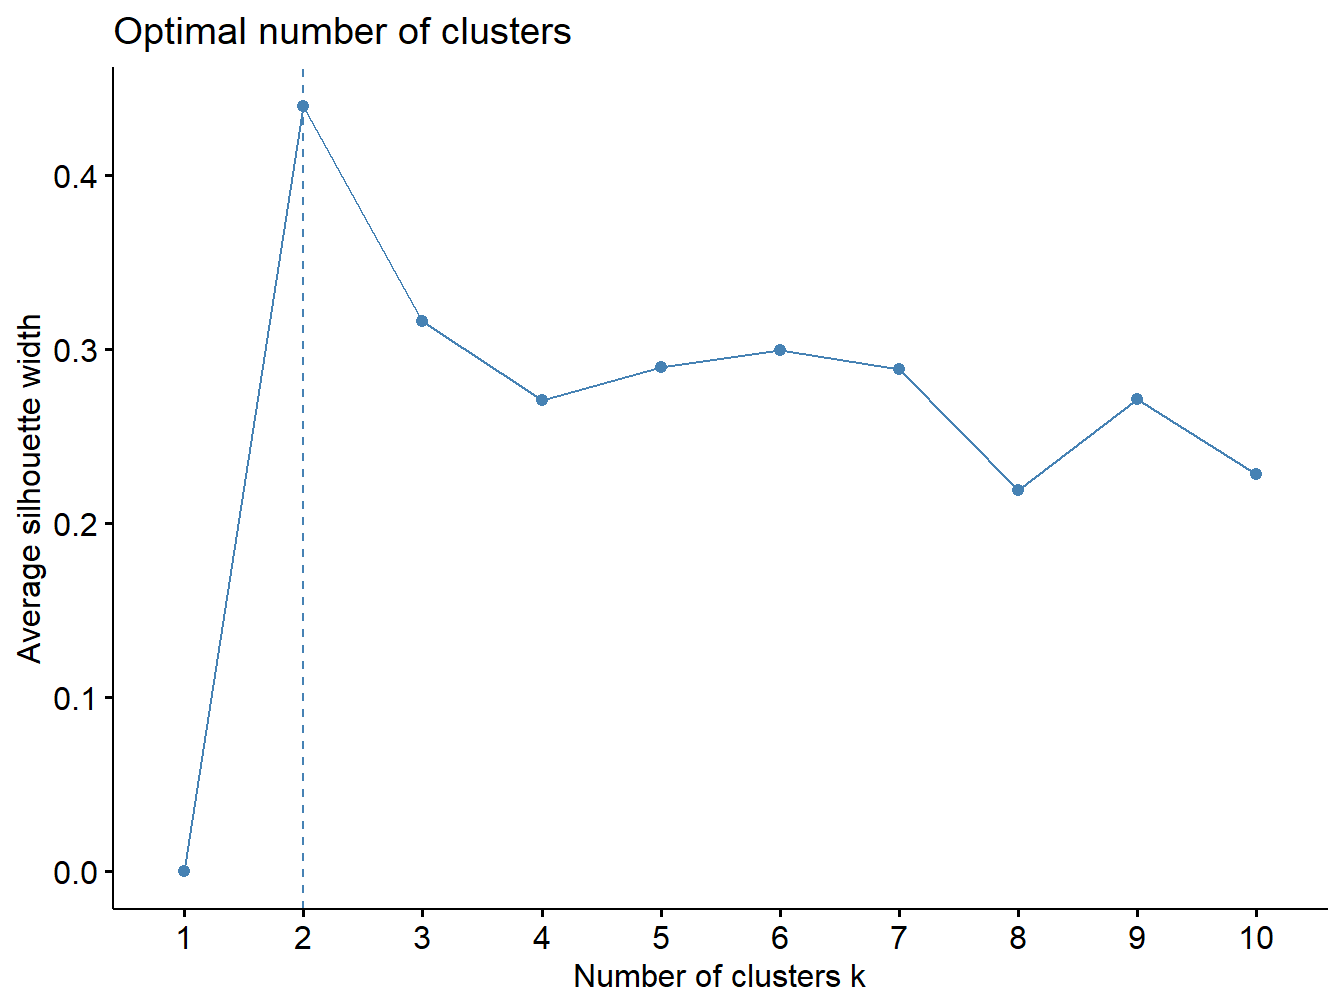
\includegraphics[width=0.8\linewidth]{01-KM_files/figure-latex/unnamed-chunk-7-1} 

}

\caption{Plot Jumlah Cluster Metode silhouette}\label{fig:unnamed-chunk-7}
\end{figure}

Pendekatan rata-rata nilai metode silhouette untuk menduga kualitas dari klaster yang terbentuk. Semakin tinggi nilai rata-ratanya maka akan semakin baik. Berdasarkan grafik pada gambar di atas banyak klaster optimal yang terbentuk pada 𝐾 = 2.

\hypertarget{eksperimen-k-means-clustering}{%
\subsection{Eksperimen K-Means Clustering}\label{eksperimen-k-means-clustering}}

Dari pendekatan metode elbow dan metode Silhouette di dapatkan jumlah \emph{cluster} optimal adalah K=2. setelah ini dilakukan eksperimen jumlah K=2

\begin{Shaded}
\begin{Highlighting}[]
\CommentTok{\#Computing k{-}means clustering}
\CommentTok{\#Compute k{-}means with k = 2}
\FunctionTok{set.seed}\NormalTok{(}\DecValTok{123}\NormalTok{)}
\NormalTok{km.res }\OtherTok{\textless{}{-}} \FunctionTok{kmeans}\NormalTok{(data, }\DecValTok{2}\NormalTok{, }\AttributeTok{nstart =} \DecValTok{25}\NormalTok{)}
\CommentTok{\# Print the results}
\FunctionTok{print}\NormalTok{(km.res)}
\end{Highlighting}
\end{Shaded}

\begin{verbatim}
## K-means clustering with 2 clusters of sizes 22, 13
## 
## Cluster means:
##         X1       X2       X3       X4       X5       X6       X7
## 1 1.918182 2.017273 1.675000 1.949091 1.890455 1.728182 1.557273
## 2 4.446923 4.276923 4.854615 4.394615 4.494615 4.769231 5.056154
##         X8       X9      X10
## 1 1.286818 1.952727 1.455455
## 2 5.515385 4.389231 5.230000
## 
## Clustering vector:
##         CILACAP        BANYUMAS     PURBALINGGA    BANJARNEGARA 
##               2               2               2               2 
##         KEBUMEN       PURWOREJO        WONOSOBO        MAGELANG 
##               2               1               1               2 
##        BOYOLALI          KLATEN       SUKOHARJO        WONOGIRI 
##               1               2               1               1 
##     KARANGANYAR          SRAGEN        GROBOGAN           BLORA 
##               1               1               2               1 
##         REMBANG            PATI           KUDUS          JEPARA 
##               1               2               1               2 
##         DEMAK          SEMARANG      TEMANGGUNG          KENDAL 
##               1               1               1               1 
##          BATANG      PEKALONGAN        PEMALANG           TEGAL 
##               1               1               2               2 
##          BREBES   KOTA MAGELANG  KOTA SURAKARTA   KOTA SALATIGA 
##               2               1               1               1 
##   KOTA SEMARANG KOTA PEKALONGAN      KOTA TEGAL 
##               1               1               1 
## 
## Within cluster sum of squares by cluster:
## [1] 262.6536 466.0163
##  (between_SS / total_SS =  51.3 %)
## 
## Available components:
## 
## [1] "cluster"      "centers"      "totss"        "withinss"    
## [5] "tot.withinss" "betweenss"    "size"         "iter"        
## [9] "ifault"
\end{verbatim}

Melihat hasil \emph{cluster} akhir pada setiap kabupaten

\begin{Shaded}
\begin{Highlighting}[]
\CommentTok{\# Cluster number for each of the observations}
\NormalTok{km.res}\SpecialCharTok{$}\NormalTok{cluster}
\end{Highlighting}
\end{Shaded}

\begin{verbatim}
##         CILACAP        BANYUMAS     PURBALINGGA    BANJARNEGARA 
##               2               2               2               2 
##         KEBUMEN       PURWOREJO        WONOSOBO        MAGELANG 
##               2               1               1               2 
##        BOYOLALI          KLATEN       SUKOHARJO        WONOGIRI 
##               1               2               1               1 
##     KARANGANYAR          SRAGEN        GROBOGAN           BLORA 
##               1               1               2               1 
##         REMBANG            PATI           KUDUS          JEPARA 
##               1               2               1               2 
##         DEMAK          SEMARANG      TEMANGGUNG          KENDAL 
##               1               1               1               1 
##          BATANG      PEKALONGAN        PEMALANG           TEGAL 
##               1               1               2               2 
##          BREBES   KOTA MAGELANG  KOTA SURAKARTA   KOTA SALATIGA 
##               2               1               1               1 
##   KOTA SEMARANG KOTA PEKALONGAN      KOTA TEGAL 
##               1               1               1
\end{verbatim}

Melihat jumlah anggota \emph{cluster}

\begin{Shaded}
\begin{Highlighting}[]
\CommentTok{\# Cluster size}
\NormalTok{km.res}\SpecialCharTok{$}\NormalTok{size}
\end{Highlighting}
\end{Shaded}

\begin{verbatim}
## [1] 22 13
\end{verbatim}

\hypertarget{visualisasi-hasil-clustering}{%
\subsection{\texorpdfstring{Visualisasi Hasil \emph{clustering}}{Visualisasi Hasil clustering}}\label{visualisasi-hasil-clustering}}

\begin{Shaded}
\begin{Highlighting}[]
\CommentTok{\# Cluster means}
\NormalTok{km.res}\SpecialCharTok{$}\NormalTok{centers}
\end{Highlighting}
\end{Shaded}

\begin{verbatim}
##         X1       X2       X3       X4       X5       X6       X7
## 1 1.918182 2.017273 1.675000 1.949091 1.890455 1.728182 1.557273
## 2 4.446923 4.276923 4.854615 4.394615 4.494615 4.769231 5.056154
##         X8       X9      X10
## 1 1.286818 1.952727 1.455455
## 2 5.515385 4.389231 5.230000
\end{verbatim}

\begin{Shaded}
\begin{Highlighting}[]
\FunctionTok{fviz\_cluster}\NormalTok{(km.res, }\AttributeTok{data =}\NormalTok{ data)}
\end{Highlighting}
\end{Shaded}

\begin{figure}

{\centering \includegraphics[width=0.8\linewidth]{01-KM_files/figure-latex/unnamed-chunk-11-1} 

}

\caption{Plot Hasil Cluster}\label{fig:unnamed-chunk-11}
\end{figure}

\begin{Shaded}
\begin{Highlighting}[]
\FunctionTok{fviz\_cluster}\NormalTok{(km.res, }\AttributeTok{data =}\NormalTok{ data,}
             \AttributeTok{palette =} \FunctionTok{c}\NormalTok{(}\StringTok{"\#FC4E07"}\NormalTok{, }\StringTok{"\#00AFBB"}\NormalTok{),}
             \AttributeTok{ellipse.type =} \StringTok{"euclid"}\NormalTok{, }\CommentTok{\# Concentration ellipse}
             \AttributeTok{star.plot =} \ConstantTok{TRUE}\NormalTok{, }\CommentTok{\# Add segments from centroids to items}
             \AttributeTok{repel =} \ConstantTok{TRUE}\NormalTok{, }\CommentTok{\# Avoid label overplotting (slow)}
             \AttributeTok{ggtheme =} \FunctionTok{theme\_minimal}\NormalTok{())}
\end{Highlighting}
\end{Shaded}

\begin{figure}

{\centering \includegraphics[width=0.8\linewidth]{01-KM_files/figure-latex/unnamed-chunk-12-1} 

}

\caption{Plot Hasil Cluster}\label{fig:unnamed-chunk-12}
\end{figure}

\hypertarget{algoritma-fuzzy-c-means}{%
\chapter{Algoritma Fuzzy C-Means}\label{algoritma-fuzzy-c-means}}

\hypertarget{pengantar-algoritma-fuzzy-c-means}{%
\section{Pengantar Algoritma Fuzzy C-Means}\label{pengantar-algoritma-fuzzy-c-means}}

Fuzzy c-means merupakan metode yang dikenal baik dalam mendeteksi klaster (\protect\hyperlink{ref-pimentel2016}{Pimentel and Souza 2016}). Metode ini menggunakan model pengelompokan fuzzy sehingga data dapat menjadi anggota dari semua kelas atau klaster terbentuk dengan derajat atau tingkat keanggotaan yang berbeda antara 0 hingga 1. Tingkat keberadaan data dalam suatu kelas atau klaster ditentukan oleh derajat keanggotaannya. Kelebihan dari metode ini adalah penempatan pusat klaster yang lebih tepat dibandingkan dengan metode lain. Caranya adalah dengan memperbaiki pusat klaster secara berulang, maka akan dapat dilihat bahwa pusat klaster akan bergerak menuju lokasi yang tepat (Wijaya, 2014). Namun, pada algoritma Fuzzy c-means dibutuhkan waktu komputasi yang lama (\protect\hyperlink{ref-stetco2015}{Stetco, Zeng, and Keane 2015}).

Klastering dengan algoritma Fuzzy C-Means didasarkan pada teori logika fuzzy yang diperkenalkan oleh Lotfi Zadeh pada tahun 1965 dengan nama himpunan fuzzy (fuzzy set). Fuzzy C-Means Clustering pertama kali diperkenalkan oleh Dun pada (1973) dan diperbaiki oleh Bezdek (\protect\hyperlink{ref-bezdek1984}{Bezdek, Ehrlich, and Full 1984}). Dalam teori fuzzy, keangotaan sebuah data diberikan dengan suatu nilai derajat keanggotaan yang jangkauan nilainya 0 sampai 1. Semakin tinggi nilai derajat keanggotaannya maka semakin tinggi nilai keanggotaan sebuah data dalam suatu kelompok dan semakin kecil nilai derajat keanggotaannya maka semakin rendah nilai keanggotaan sebuah data dalam suatu kelompok.

Asumsikan terdapat sejumlah data dalam dataset \(X\) yang berisi \(n\) data yang dinotasikan \(X={x_1,x_2, …,x_n}\), dimana setiap data mempunyai fitur \(r\) dimensi: \(x_{i1}, x_{i2}, ..., x_{ir}\), dinotasikan \(x_i={x_i1, x_i2, ..., x_ir}\). Ada sejumlah klaster \(C\) dengan centroid: \(C_1, C_2, ..., C_k\), dimana \(k\) adalah jumlah klaster. Setiap data mempunyai derajat keanggotaan pada setiap klaster, dinyatakan dengan \(u_{ij}\), dengan nilai diantara 0 dan 1, \(i\) menyatakan data \(x_i\) dan \(j\) menyatakan klaster \(c_j\). Jumlah nilai derajat keanggotaan setiap data \(x_i\) selalu sama dengan 1, yang diformulasikan pada persamaan berikut:

\begin{theorem}
\protect\hypertarget{thm:unnamed-chunk-1}{}\label{thm:unnamed-chunk-1}\[\sum_{j=1}^k u_{i j}=1\]
\end{theorem}

Fuzzy c-means clustering merupakan suatu metode clustering yang hampir mirip seperti k-means clustering. Karena metode clustering ini mirip dengan k-means clustering, ada yang menyebut metode ini fuzzy k-means clustering. Fuzzy c-means merupakan salah satu jenis soft clustering dimana dalam mengelompokan suatu data, setiap data bisa dimiliki lebih dari satu cluster.

Cara kerja dari fuzzy c-means clustering dalam mengelompokkan datanya adalah sebagai berikut :

\begin{enumerate}
\def\labelenumi{\arabic{enumi}.}
\item
  Menentukan banyak cluster (k) yang akan dibuat.
\item
  Menentukan nilai proporsi untuk setiap data poin secara random untuk masuk dalam suatu cluster. Menghitung nilai centroid.
\item
  Dalam menghitung nilai centroid, kita menggunakan formula berikut:
\end{enumerate}

\begin{lemma}
\protect\hypertarget{lem:unnamed-chunk-2}{}\label{lem:unnamed-chunk-2}\[C_j=\frac{\sum{{\mu }^m_{ij}}x}{\sum{{\mu }^m_{ij}}}\]
\end{lemma}

\begin{enumerate}
\def\labelenumi{\arabic{enumi}.}
\setcounter{enumi}{3}
\tightlist
\item
  Menghtung kembali nilai proporsi untuk setiap data poin untuk masuk pada setiap cluster. formula yang digunakan yaitu sebagai berikut:
\end{enumerate}

\begin{lemma}
\protect\hypertarget{lem:unnamed-chunk-3}{}\label{lem:unnamed-chunk-3}\[{\mu }^m_{ij}=\frac{1}{\sum{{\left(\frac{\left|x_i-c_j\right|}{\left|x_i-c_k\right|}\right)}^{\frac{2}{m-1}}}}\]
\end{lemma}

\hypertarget{eksperimeen-fuzzy-c-means}{%
\section{Eksperimeen Fuzzy C-Means}\label{eksperimeen-fuzzy-c-means}}

\hypertarget{install-dan-load-packagaes}{%
\subsection{Install dan Load Packagaes}\label{install-dan-load-packagaes}}

\begin{Shaded}
\begin{Highlighting}[]
\FunctionTok{library}\NormalTok{(ppclust)}
\FunctionTok{library}\NormalTok{(factoextra)}
\FunctionTok{library}\NormalTok{(fclust)}
\FunctionTok{library}\NormalTok{(cluster)}
\end{Highlighting}
\end{Shaded}

\hypertarget{data-1}{%
\subsection{Data}\label{data-1}}

\begin{Shaded}
\begin{Highlighting}[]
\FunctionTok{library}\NormalTok{ (readr)}
\NormalTok{urlfile }\OtherTok{=} \StringTok{"https://raw.githubusercontent.com/dedenistiawan/Dataset/main/Basis\%20Data\%20Terpadu\%20Jateng.csv"}

\NormalTok{data}\OtherTok{\textless{}{-}}\FunctionTok{read.csv}\NormalTok{(}\FunctionTok{url}\NormalTok{(urlfile), }\AttributeTok{row.names =} \StringTok{"Kabupaten"}\NormalTok{)}
\end{Highlighting}
\end{Shaded}

\hypertarget{hasil-clustering}{%
\subsection{Hasil Clustering}\label{hasil-clustering}}

\begin{Shaded}
\begin{Highlighting}[]
\FunctionTok{library}\NormalTok{(ppclust)}
\NormalTok{res.fcm }\OtherTok{\textless{}{-}} \FunctionTok{fcm}\NormalTok{(data, }\AttributeTok{centers=}\DecValTok{3}\NormalTok{)}
\FunctionTok{as.data.frame}\NormalTok{(res.fcm}\SpecialCharTok{$}\NormalTok{u)}
\end{Highlighting}
\end{Shaded}

\begin{verbatim}
##                  Cluster 1  Cluster 2  Cluster 3
## CILACAP         0.09432155 0.70608174 0.19959671
## BANYUMAS        0.03242738 0.87685700 0.09071562
## PURBALINGGA     0.12503329 0.58855259 0.28641412
## BANJARNEGARA    0.15770912 0.27431153 0.56797934
## KEBUMEN         0.12183017 0.55326811 0.32490172
## PURWOREJO       0.37665821 0.15508384 0.46825795
## WONOSOBO        0.73997169 0.04794255 0.21208577
## MAGELANG        0.12565978 0.11864932 0.75569090
## BOYOLALI        0.65917928 0.04746322 0.29335751
## KLATEN          0.15366683 0.40625017 0.44008300
## SUKOHARJO       0.90659203 0.01812578 0.07528219
## WONOGIRI        0.62649398 0.05984340 0.31366262
## KARANGANYAR     0.83280963 0.03151333 0.13567704
## SRAGEN          0.92987167 0.01369224 0.05643609
## GROBOGAN        0.10906165 0.20509357 0.68584478
## BLORA           0.42364979 0.06584083 0.51050938
## REMBANG         0.77496097 0.03515460 0.18988443
## PATI            0.18226626 0.18018760 0.63754615
## KUDUS           0.93999864 0.01358093 0.04642043
## JEPARA          0.13357477 0.17434136 0.69208387
## DEMAK           0.22405973 0.12077163 0.65516864
## SEMARANG        0.92443899 0.01375558 0.06180543
## TEMANGGUNG      0.92181846 0.01515432 0.06302723
## KENDAL          0.30783534 0.07103512 0.62112953
## BATANG          0.74568211 0.05146780 0.20285008
## PEKALONGAN      0.33879435 0.11753007 0.54367557
## PEMALANG        0.13508254 0.47108349 0.39383397
## TEGAL           0.08391671 0.61445746 0.30162583
## BREBES          0.11958050 0.64100931 0.23941019
## KOTA MAGELANG   0.82227544 0.05127744 0.12644712
## KOTA SURAKARTA  0.88284897 0.03051218 0.08663885
## KOTA SALATIGA   0.82356236 0.05093432 0.12550332
## KOTA SEMARANG   0.81177689 0.04152177 0.14670134
## KOTA PEKALONGAN 0.87988142 0.03226874 0.08784985
## KOTA TEGAL      0.88100104 0.03188749 0.08711147
\end{verbatim}

\begin{Shaded}
\begin{Highlighting}[]
\CommentTok{\# Visualize using corrplot}
\FunctionTok{library}\NormalTok{(corrplot)}
\end{Highlighting}
\end{Shaded}

\begin{verbatim}
## corrplot 0.92 loaded
\end{verbatim}

\begin{Shaded}
\begin{Highlighting}[]
\FunctionTok{corrplot}\NormalTok{(res.fcm}\SpecialCharTok{$}\NormalTok{u, }\AttributeTok{is.corr =} \ConstantTok{FALSE}\NormalTok{)}
\end{Highlighting}
\end{Shaded}

\includegraphics{02-FCM_files/figure-latex/unnamed-chunk-6-1.pdf}

\begin{Shaded}
\begin{Highlighting}[]
\NormalTok{res.fcm}\SpecialCharTok{$}\NormalTok{v0}
\end{Highlighting}
\end{Shaded}

\begin{verbatim}
##             X1   X2   X3   X4   X5   X6   X7   X8   X9  X10
## Cluster 1 1.52 1.69 1.59 1.68 1.91 1.39 0.37 0.13 0.86 0.52
## Cluster 2 5.71 4.47 5.18 5.51 5.02 6.21 7.39 6.96 5.98 8.22
## Cluster 3 4.78 3.91 6.70 4.84 6.35 5.82 3.00 5.99 2.98 5.98
\end{verbatim}

\begin{Shaded}
\begin{Highlighting}[]
\NormalTok{res.fcm}\SpecialCharTok{$}\NormalTok{v}
\end{Highlighting}
\end{Shaded}

\begin{verbatim}
##                 X1       X2       X3       X4       X5       X6
## Cluster 1 1.724771 1.743303 1.432408 1.706002 1.626688 1.504833
## Cluster 2 5.001721 4.041093 5.531054 4.669414 4.638562 5.500335
## Cluster 3 3.418238 4.025821 3.497306 3.657048 3.843888 3.477061
##                 X7       X8       X9      X10
## Cluster 1 1.335312 1.021470 1.697120 1.056498
## Cluster 2 6.458007 7.009924 4.458629 6.474407
## Cluster 3 3.074419 3.057133 3.802309 3.529256
\end{verbatim}

\hypertarget{hasil-clustering-fcm}{%
\subsection{Hasil Clustering FCM}\label{hasil-clustering-fcm}}

\begin{Shaded}
\begin{Highlighting}[]
\FunctionTok{summary}\NormalTok{(res.fcm)}
\end{Highlighting}
\end{Shaded}

\begin{verbatim}
## Summary for 'res.fcm'
## 
## Number of data objects:  35 
## 
## Number of clusters:  3 
## 
## Crisp clustering vector:
##  [1] 2 2 2 3 2 3 1 3 1 3 1 1 1 1 3 3 1 3 1 3 3 1 1 3 1 3 2 2 2 1 1 1
## [33] 1 1 1
## 
## Initial cluster prototypes:
##             X1   X2   X3   X4   X5   X6   X7   X8   X9  X10
## Cluster 1 1.52 1.69 1.59 1.68 1.91 1.39 0.37 0.13 0.86 0.52
## Cluster 2 5.71 4.47 5.18 5.51 5.02 6.21 7.39 6.96 5.98 8.22
## Cluster 3 4.78 3.91 6.70 4.84 6.35 5.82 3.00 5.99 2.98 5.98
## 
## Final cluster prototypes:
##                 X1       X2       X3       X4       X5       X6
## Cluster 1 1.724771 1.743303 1.432408 1.706002 1.626688 1.504833
## Cluster 2 5.001721 4.041093 5.531054 4.669414 4.638562 5.500335
## Cluster 3 3.418238 4.025821 3.497306 3.657048 3.843888 3.477061
##                 X7       X8       X9      X10
## Cluster 1 1.335312 1.021470 1.697120 1.056498
## Cluster 2 6.458007 7.009924 4.458629 6.474407
## Cluster 3 3.074419 3.057133 3.802309 3.529256
## 
## Distance between the final cluster prototypes
##           Cluster 1 Cluster 2
## Cluster 2 165.71763          
## Cluster 3  42.66853  48.57171
## 
## Difference between the initial and final cluster prototypes
##                   X1          X2         X3          X4         X5
## Cluster 1  0.2047706  0.05330275 -0.1575916  0.02600226 -0.2833119
## Cluster 2 -0.7082786 -0.42890656  0.3510540 -0.84058553 -0.3814383
## Cluster 3 -1.3617618  0.11582102 -3.2026942 -1.18295161 -2.5061115
##                   X6          X7          X8         X9        X10
## Cluster 1  0.1148330  0.96531199  0.89147037  0.8371205  0.5364979
## Cluster 2 -0.7096647 -0.93199283  0.04992404 -1.5213711 -1.7455932
## Cluster 3 -2.3429386  0.07441915 -2.93286736  0.8223093 -2.4507443
## 
## Root Mean Squared Deviations (RMSD): 4.157732 
## Mean Absolute Deviation (MAD): 95.77214 
## 
## Membership degrees matrix (top and bottom 5 rows): 
##               Cluster 1 Cluster 2  Cluster 3
## CILACAP      0.09432155 0.7060817 0.19959671
## BANYUMAS     0.03242738 0.8768570 0.09071562
## PURBALINGGA  0.12503329 0.5885526 0.28641412
## BANJARNEGARA 0.15770912 0.2743115 0.56797934
## KEBUMEN      0.12183017 0.5532681 0.32490172
## ...
##                 Cluster 1  Cluster 2  Cluster 3
## KOTA SURAKARTA  0.8828490 0.03051218 0.08663885
## KOTA SALATIGA   0.8235624 0.05093432 0.12550332
## KOTA SEMARANG   0.8117769 0.04152177 0.14670134
## KOTA PEKALONGAN 0.8798814 0.03226873 0.08784985
## KOTA TEGAL      0.8810010 0.03188749 0.08711147
## 
## Descriptive statistics for the membership degrees by clusters
##           Size       Min        Q1      Mean    Median        Q3
## Cluster 1   17 0.6264940 0.7749610 0.8295979 0.8328096 0.9065920
## Cluster 2    7 0.4710835 0.5709104 0.6359014 0.6144575 0.6735455
## Cluster 3   11 0.4400830 0.5270925 0.5979972 0.6211295 0.6705067
##                 Max
## Cluster 1 0.9399986
## Cluster 2 0.8768570
## Cluster 3 0.7556909
## 
## Dunn's Fuzziness Coefficients:
## dunn_coeff normalized 
##  0.5999684  0.3999525 
## 
## Within cluster sum of squares by cluster:
##        1        2        3 
## 130.5953 220.3251 200.0818 
## (between_SS / total_SS =  61.98%) 
## 
## Available components: 
##  [1] "u"          "v"          "v0"         "d"          "x"         
##  [6] "cluster"    "csize"      "sumsqrs"    "k"          "m"         
## [11] "iter"       "best.start" "func.val"   "comp.time"  "inpargs"   
## [16] "algorithm"  "call"
\end{verbatim}

\hypertarget{run-fcm-with-multiple-starts}{%
\subsection{Run FCM with Multiple Starts}\label{run-fcm-with-multiple-starts}}

\begin{Shaded}
\begin{Highlighting}[]
\NormalTok{res.fcm }\OtherTok{\textless{}{-}} \FunctionTok{fcm}\NormalTok{(data, }\AttributeTok{centers=}\DecValTok{3}\NormalTok{, }\AttributeTok{nstart=}\DecValTok{5}\NormalTok{)}
\end{Highlighting}
\end{Shaded}

\begin{Shaded}
\begin{Highlighting}[]
\NormalTok{res.fcm }\OtherTok{\textless{}{-}} \FunctionTok{fcm}\NormalTok{(data, }\AttributeTok{centers=}\DecValTok{3}\NormalTok{, }\AttributeTok{nstart=}\DecValTok{5}\NormalTok{, }\AttributeTok{fixmemb=}\ConstantTok{TRUE}\NormalTok{)}
\end{Highlighting}
\end{Shaded}

\hypertarget{display-the-best-solution}{%
\subsection{Display the best solution}\label{display-the-best-solution}}

\begin{Shaded}
\begin{Highlighting}[]
\NormalTok{res.fcm}\SpecialCharTok{$}\NormalTok{func.val}
\end{Highlighting}
\end{Shaded}

\begin{verbatim}
## [1] 360.931 360.931 360.931 360.931 360.931
\end{verbatim}

\begin{Shaded}
\begin{Highlighting}[]
\NormalTok{res.fcm}\SpecialCharTok{$}\NormalTok{iter}
\end{Highlighting}
\end{Shaded}

\begin{verbatim}
## [1] 74 74 74 75 77
\end{verbatim}

\begin{Shaded}
\begin{Highlighting}[]
\NormalTok{res.fcm}\SpecialCharTok{$}\NormalTok{best.start}
\end{Highlighting}
\end{Shaded}

\begin{verbatim}
## [1] 1
\end{verbatim}

\hypertarget{display-the-summary-of-clustering-results}{%
\subsection{Display the summary of clustering results}\label{display-the-summary-of-clustering-results}}

\begin{Shaded}
\begin{Highlighting}[]
\FunctionTok{summary}\NormalTok{(res.fcm)}
\end{Highlighting}
\end{Shaded}

\begin{verbatim}
## Summary for 'res.fcm'
## 
## Number of data objects:  35 
## 
## Number of clusters:  3 
## 
## Crisp clustering vector:
##  [1] 3 3 3 2 3 2 1 2 1 2 1 1 1 1 2 2 1 2 1 2 2 1 1 2 1 2 3 3 3 1 1 1
## [33] 1 1 1
## 
## Initial cluster prototypes:
##             X1   X2   X3   X4   X5   X6   X7   X8   X9  X10
## Cluster 1 2.13 1.95 3.00 1.78 1.62 2.06 0.45 2.32 3.57 0.84
## Cluster 2 3.84 5.15 1.93 4.64 4.04 3.78 8.71 4.45 3.99 3.09
## Cluster 3 3.99 6.35 3.16 5.52 5.77 4.28 3.84 0.02 3.88 2.82
## 
## Final cluster prototypes:
##                 X1       X2       X3       X4       X5       X6
## Cluster 1 1.724771 1.743303 1.432408 1.706002 1.626688 1.504833
## Cluster 2 3.418238 4.025821 3.497306 3.657048 3.843888 3.477061
## Cluster 3 5.001721 4.041093 5.531054 4.669414 4.638562 5.500335
##                 X7       X8       X9      X10
## Cluster 1 1.335312 1.021470 1.697120 1.056498
## Cluster 2 3.074419 3.057133 3.802309 3.529256
## Cluster 3 6.458007 7.009924 4.458629 6.474407
## 
## Distance between the final cluster prototypes
##           Cluster 1 Cluster 2
## Cluster 2  42.66853          
## Cluster 3 165.71763  48.57171
## 
## Difference between the initial and final cluster prototypes
##                   X1         X2        X3          X4           X5
## Cluster 1 -0.4052294 -0.2066973 -1.567592 -0.07399774  0.006688052
## Cluster 2 -0.4217618 -1.1241790  1.567306 -0.98295161 -0.196111507
## Cluster 3  1.0117214 -2.3089066  2.371054 -0.85058553 -1.131438314
##                   X6        X7        X8         X9       X10
## Cluster 1 -0.5551670  0.885312 -1.298530 -1.8728795 0.2164979
## Cluster 2 -0.3029386 -5.635581 -1.392867 -0.1876907 0.4392557
## Cluster 3  1.2203353  2.618007  6.989924  0.5786289 3.6544068
## 
## Root Mean Squared Deviations (RMSD): 6.653244 
## Mean Absolute Deviation (MAD): 140.2475 
## 
## Membership degrees matrix (top and bottom 5 rows): 
##               Cluster 1  Cluster 2 Cluster 3
## CILACAP      0.09432155 0.19959671 0.7060817
## BANYUMAS     0.03242738 0.09071562 0.8768570
## PURBALINGGA  0.12503329 0.28641412 0.5885526
## BANJARNEGARA 0.15770912 0.56797934 0.2743115
## KEBUMEN      0.12183017 0.32490172 0.5532681
## ...
##                 Cluster 1  Cluster 2  Cluster 3
## KOTA SURAKARTA  0.8828490 0.08663885 0.03051218
## KOTA SALATIGA   0.8235624 0.12550332 0.05093432
## KOTA SEMARANG   0.8117769 0.14670134 0.04152177
## KOTA PEKALONGAN 0.8798814 0.08784985 0.03226873
## KOTA TEGAL      0.8810010 0.08711147 0.03188749
## 
## Descriptive statistics for the membership degrees by clusters
##           Size       Min        Q1      Mean    Median        Q3
## Cluster 1   17 0.6264940 0.7749610 0.8295979 0.8328096 0.9065920
## Cluster 2   11 0.4400830 0.5270925 0.5979972 0.6211295 0.6705067
## Cluster 3    7 0.4710835 0.5709104 0.6359014 0.6144575 0.6735455
##                 Max
## Cluster 1 0.9399986
## Cluster 2 0.7556909
## Cluster 3 0.8768570
## 
## Dunn's Fuzziness Coefficients:
## dunn_coeff normalized 
##  0.5999684  0.3999525 
## 
## Within cluster sum of squares by cluster:
##        1        2        3 
## 130.5953 200.0818 220.3251 
## (between_SS / total_SS =  61.98%) 
## 
## Available components: 
##  [1] "u"          "v"          "v0"         "d"          "x"         
##  [6] "cluster"    "csize"      "sumsqrs"    "k"          "m"         
## [11] "iter"       "best.start" "func.val"   "comp.time"  "inpargs"   
## [16] "algorithm"  "call"
\end{verbatim}

\hypertarget{cluster-plot-with-fviz_cluster}{%
\subsection{Cluster Plot with fviz\_cluster}\label{cluster-plot-with-fviz_cluster}}

\begin{Shaded}
\begin{Highlighting}[]
\NormalTok{res.fcm2 }\OtherTok{\textless{}{-}} \FunctionTok{ppclust2}\NormalTok{(res.fcm, }\StringTok{"kmeans"}\NormalTok{)}
\NormalTok{factoextra}\SpecialCharTok{::}\FunctionTok{fviz\_cluster}\NormalTok{(res.fcm2, }\AttributeTok{data =}\NormalTok{ data, }
  \AttributeTok{ellipse.type =} \StringTok{"convex"}\NormalTok{,}
  \AttributeTok{palette =} \StringTok{"jco"}\NormalTok{,}
  \AttributeTok{repel =} \ConstantTok{TRUE}\NormalTok{)}
\end{Highlighting}
\end{Shaded}

\includegraphics{02-FCM_files/figure-latex/unnamed-chunk-16-1.pdf}

\hypertarget{cluster-plot-with-clusplot}{%
\subsection{Cluster Plot with clusplot}\label{cluster-plot-with-clusplot}}

\begin{Shaded}
\begin{Highlighting}[]
\NormalTok{res.fcm3 }\OtherTok{\textless{}{-}} \FunctionTok{ppclust2}\NormalTok{(res.fcm, }\StringTok{"fanny"}\NormalTok{)}

\NormalTok{cluster}\SpecialCharTok{::}\FunctionTok{clusplot}\NormalTok{(}\FunctionTok{scale}\NormalTok{(data), res.fcm3}\SpecialCharTok{$}\NormalTok{cluster,  }
  \AttributeTok{main =} \StringTok{"Cluster plot of Iris data set"}\NormalTok{,}
  \AttributeTok{color=}\ConstantTok{TRUE}\NormalTok{, }\AttributeTok{labels =} \DecValTok{2}\NormalTok{, }\AttributeTok{lines =} \DecValTok{2}\NormalTok{, }\AttributeTok{cex=}\DecValTok{1}\NormalTok{)}
\end{Highlighting}
\end{Shaded}

\includegraphics{02-FCM_files/figure-latex/unnamed-chunk-17-1.pdf}

\hypertarget{metode-cluster-hirarki}{%
\chapter{Metode Cluster Hirarki}\label{metode-cluster-hirarki}}

\hypertarget{data-2}{%
\section{Data}\label{data-2}}

\begin{Shaded}
\begin{Highlighting}[]
\FunctionTok{library}\NormalTok{ (readr)}
\NormalTok{urlfile }\OtherTok{=} \StringTok{"https://raw.githubusercontent.com/dedenistiawan/Dataset/main/Basis\%20Data\%20Terpadu\%20Jateng.csv"}

\NormalTok{data}\OtherTok{\textless{}{-}}\FunctionTok{read.csv}\NormalTok{(}\FunctionTok{url}\NormalTok{(urlfile), }\AttributeTok{row.names =} \StringTok{"Kabupaten"}\NormalTok{)}
\end{Highlighting}
\end{Shaded}

\begin{Shaded}
\begin{Highlighting}[]
\NormalTok{knitr}\SpecialCharTok{::}\FunctionTok{kable}\NormalTok{(}
  \FunctionTok{head}\NormalTok{(data, }\DecValTok{10}\NormalTok{), }\AttributeTok{caption =} \StringTok{\textquotesingle{}Basis Data Terpadu Jawa Tengah\textquotesingle{}}\NormalTok{,}
  \AttributeTok{booktabs =} \ConstantTok{TRUE}\NormalTok{)}
\end{Highlighting}
\end{Shaded}

\begin{longtable}[]{@{}lrrrrrrrrrr@{}}
\caption{\label{tab:nice-tab}Basis Data Terpadu Jawa Tengah}\tabularnewline
\toprule\noalign{}
& X1 & X2 & X3 & X4 & X5 & X6 & X7 & X8 & X9 & X10 \\
\midrule\noalign{}
\endfirsthead
\toprule\noalign{}
& X1 & X2 & X3 & X4 & X5 & X6 & X7 & X8 & X9 & X10 \\
\midrule\noalign{}
\endhead
\bottomrule\noalign{}
\endlastfoot
CILACAP & 5.19 & 5.67 & 5.08 & 5.44 & 5.22 & 6.05 & 11.47 & 9.78 & 5.55 & 5.12 \\
BANYUMAS & 5.71 & 4.47 & 5.18 & 5.51 & 5.02 & 6.21 & 7.39 & 6.96 & 5.98 & 8.22 \\
PURBALINGGA & 3.30 & 2.19 & 3.80 & 3.13 & 3.73 & 3.34 & 8.71 & 7.41 & 3.21 & 4.65 \\
BANJARNEGARA & 2.73 & 2.34 & 3.76 & 2.80 & 2.57 & 2.99 & 3.31 & 5.45 & 4.21 & 6.05 \\
KEBUMEN & 4.17 & 2.55 & 3.26 & 4.16 & 3.15 & 4.15 & 4.30 & 9.29 & 4.61 & 4.34 \\
PURWOREJO & 1.87 & 2.12 & 1.48 & 3.05 & 1.78 & 1.83 & 5.00 & 4.90 & 3.12 & 2.09 \\
WONOSOBO & 2.13 & 1.95 & 3.00 & 1.78 & 1.62 & 2.06 & 0.45 & 2.32 & 3.57 & 0.84 \\
MAGELANG & 3.95 & 3.01 & 4.22 & 4.15 & 3.01 & 3.64 & 1.44 & 3.35 & 5.69 & 3.67 \\
BOYOLALI & 2.19 & 3.07 & 1.61 & 2.74 & 2.11 & 1.82 & 1.71 & 2.34 & 3.41 & 1.55 \\
KLATEN & 3.84 & 5.15 & 1.93 & 4.64 & 4.04 & 3.78 & 8.71 & 4.45 & 3.99 & 3.09 \\
\end{longtable}

\begin{Shaded}
\begin{Highlighting}[]
\CommentTok{\# Standardize the data}
\NormalTok{df }\OtherTok{\textless{}{-}} \FunctionTok{scale}\NormalTok{(data)}
\end{Highlighting}
\end{Shaded}

\begin{Shaded}
\begin{Highlighting}[]
\CommentTok{\# Compute the dissimilarity matrix}
\CommentTok{\# df = the standardized data}
\NormalTok{res.dist }\OtherTok{\textless{}{-}} \FunctionTok{dist}\NormalTok{(df, }\AttributeTok{method =} \StringTok{"euclidean"}\NormalTok{)}
\end{Highlighting}
\end{Shaded}

\begin{Shaded}
\begin{Highlighting}[]
\FunctionTok{as.matrix}\NormalTok{(res.dist)[}\DecValTok{1}\SpecialCharTok{:}\DecValTok{5}\NormalTok{, }\DecValTok{1}\SpecialCharTok{:}\DecValTok{5}\NormalTok{]}
\end{Highlighting}
\end{Shaded}

\begin{verbatim}
##               CILACAP BANYUMAS PURBALINGGA BANJARNEGARA  KEBUMEN
## CILACAP      0.000000 2.327193    3.828424     5.188508 3.891360
## BANYUMAS     2.327193 0.000000    3.809719     4.232529 3.310710
## PURBALINGGA  3.828424 3.809719    0.000000     2.418211 2.235801
## BANJARNEGARA 5.188508 4.232529    2.418211     0.000000 2.159694
## KEBUMEN      3.891360 3.310710    2.235801     2.159694 0.000000
\end{verbatim}

\begin{Shaded}
\begin{Highlighting}[]
\NormalTok{res.hc }\OtherTok{\textless{}{-}} \FunctionTok{hclust}\NormalTok{(}\AttributeTok{d =}\NormalTok{res.dist, }\AttributeTok{method =} \StringTok{"ward.D2"}\NormalTok{)}
\end{Highlighting}
\end{Shaded}

\begin{Shaded}
\begin{Highlighting}[]
\CommentTok{\# cex: label size}
\FunctionTok{library}\NormalTok{(}\StringTok{"factoextra"}\NormalTok{)}
\end{Highlighting}
\end{Shaded}

\begin{verbatim}
## Loading required package: ggplot2
\end{verbatim}

\begin{verbatim}
## Welcome! Want to learn more? See two factoextra-related books at https://goo.gl/ve3WBa
\end{verbatim}

\begin{Shaded}
\begin{Highlighting}[]
\FunctionTok{library}\NormalTok{(ggplot2)}
\FunctionTok{fviz\_dend}\NormalTok{(res.hc, }\AttributeTok{cex =} \FloatTok{0.5}\NormalTok{)}
\end{Highlighting}
\end{Shaded}

\includegraphics{03-HC_files/figure-latex/unnamed-chunk-5-1.pdf}

\begin{Shaded}
\begin{Highlighting}[]
\CommentTok{\# Cut tree into 2 groups}
\NormalTok{grp }\OtherTok{\textless{}{-}} \FunctionTok{cutree}\NormalTok{(res.hc, }\AttributeTok{k =}\DecValTok{2}\NormalTok{)}
\FunctionTok{head}\NormalTok{(grp, }\AttributeTok{n =}\DecValTok{2}\NormalTok{)}
\end{Highlighting}
\end{Shaded}

\begin{verbatim}
##  CILACAP BANYUMAS 
##        1        1
\end{verbatim}

\begin{Shaded}
\begin{Highlighting}[]
\CommentTok{\# Number of members in each cluster}
\FunctionTok{table}\NormalTok{(grp)}
\end{Highlighting}
\end{Shaded}

\begin{verbatim}
## grp
##  1  2 
## 12 23
\end{verbatim}

\begin{Shaded}
\begin{Highlighting}[]
\CommentTok{\# Cut in 2 groups and color by groups}
\FunctionTok{fviz\_dend}\NormalTok{(res.hc, }\AttributeTok{k =}\DecValTok{2}\NormalTok{, }\CommentTok{\# Cut in four groups}
          \AttributeTok{cex =} \FloatTok{0.5}\NormalTok{, }\CommentTok{\# label size}
          \AttributeTok{k\_colors =} \FunctionTok{c}\NormalTok{(}\StringTok{"\#E7B800"}\NormalTok{, }\StringTok{"\#FC4E07"}\NormalTok{),}
          \AttributeTok{color\_labels\_by\_k =} \ConstantTok{TRUE}\NormalTok{, }\CommentTok{\# color labels by groups}
          \AttributeTok{rect =} \ConstantTok{TRUE} \CommentTok{\# Add rectangle around groups)}
\NormalTok{          )}
\end{Highlighting}
\end{Shaded}

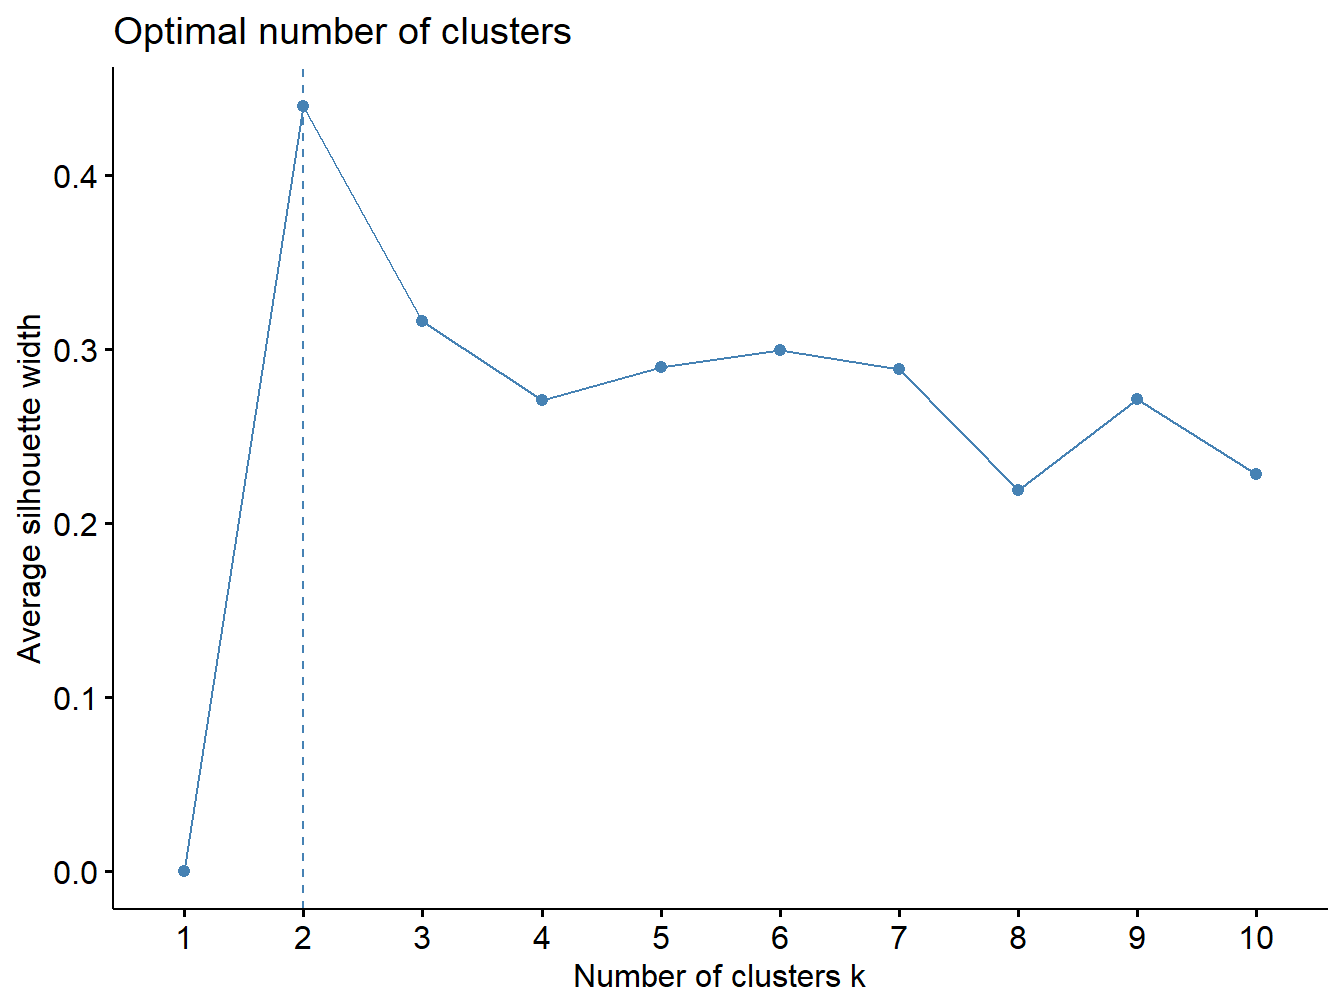
\includegraphics{03-HC_files/figure-latex/unnamed-chunk-8-1.pdf}

\begin{Shaded}
\begin{Highlighting}[]
\FunctionTok{fviz\_cluster}\NormalTok{(}\FunctionTok{list}\NormalTok{(}\AttributeTok{data =}\NormalTok{ df, }\AttributeTok{cluster =}\NormalTok{ grp),}
\AttributeTok{palette =} \FunctionTok{c}\NormalTok{(}\StringTok{"\#E7B800"}\NormalTok{, }\StringTok{"\#FC4E07"}\NormalTok{),}
\AttributeTok{ellipse.type =} \StringTok{"convex"}\NormalTok{, }\CommentTok{\# Concentration ellipse}
\AttributeTok{repel =} \ConstantTok{TRUE}\NormalTok{, }\CommentTok{\# Avoid label overplotting (slow)}
\AttributeTok{show.clust.cent =} \ConstantTok{FALSE}\NormalTok{, }\AttributeTok{ggtheme =} \FunctionTok{theme\_minimal}\NormalTok{())}
\end{Highlighting}
\end{Shaded}

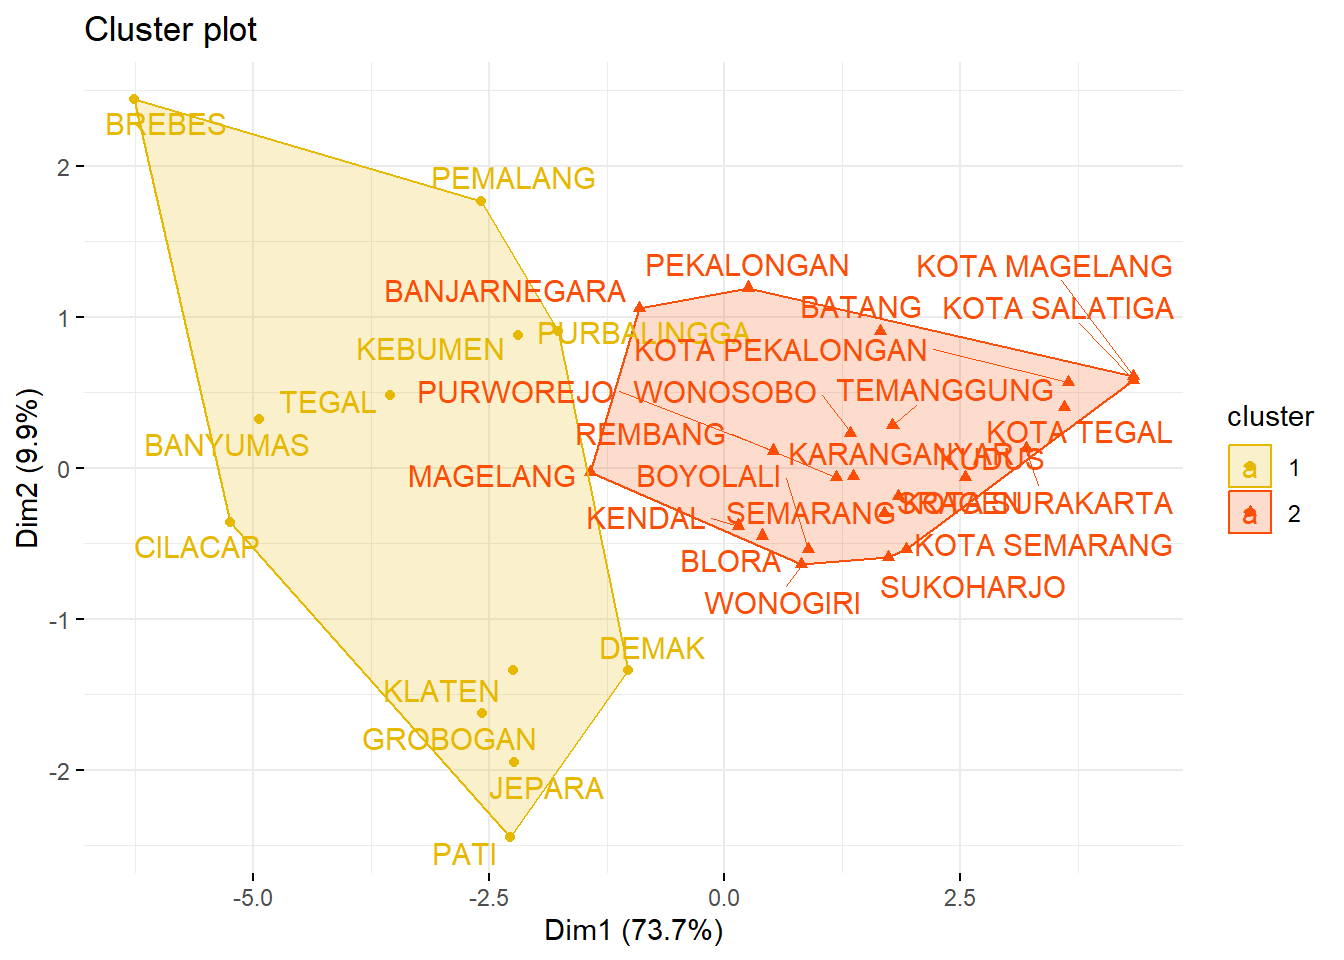
\includegraphics{03-HC_files/figure-latex/unnamed-chunk-9-1.pdf}

\hypertarget{comparing-dendrograms}{%
\section{Comparing dendrograms}\label{comparing-dendrograms}}

\begin{Shaded}
\begin{Highlighting}[]
\FunctionTok{library}\NormalTok{(dendextend)}
\end{Highlighting}
\end{Shaded}

\begin{verbatim}
## 
## ---------------------
## Welcome to dendextend version 1.17.1
## Type citation('dendextend') for how to cite the package.
## 
## Type browseVignettes(package = 'dendextend') for the package vignette.
## The github page is: https://github.com/talgalili/dendextend/
## 
## Suggestions and bug-reports can be submitted at: https://github.com/talgalili/dendextend/issues
## You may ask questions at stackoverflow, use the r and dendextend tags: 
##   https://stackoverflow.com/questions/tagged/dendextend
## 
##  To suppress this message use:  suppressPackageStartupMessages(library(dendextend))
## ---------------------
\end{verbatim}

\begin{verbatim}
## 
## Attaching package: 'dendextend'
\end{verbatim}

\begin{verbatim}
## The following object is masked from 'package:stats':
## 
##     cutree
\end{verbatim}

\begin{Shaded}
\begin{Highlighting}[]
\CommentTok{\# Compute distance matrix}
\NormalTok{res.dist }\OtherTok{\textless{}{-}} \FunctionTok{dist}\NormalTok{(df, }\AttributeTok{method =} \StringTok{"euclidean"}\NormalTok{)}

\CommentTok{\# Compute 2 hierarchical clusterings}
\NormalTok{hc1 }\OtherTok{\textless{}{-}} \FunctionTok{hclust}\NormalTok{(res.dist, }\AttributeTok{method =} \StringTok{"average"}\NormalTok{)}
\NormalTok{hc2 }\OtherTok{\textless{}{-}} \FunctionTok{hclust}\NormalTok{(res.dist, }\AttributeTok{method =} \StringTok{"ward.D2"}\NormalTok{)}

\CommentTok{\# Create two dendrograms}
\NormalTok{dend1 }\OtherTok{\textless{}{-}} \FunctionTok{as.dendrogram}\NormalTok{ (hc1)}
\NormalTok{dend2 }\OtherTok{\textless{}{-}} \FunctionTok{as.dendrogram}\NormalTok{ (hc2)}

\CommentTok{\# Create a list to hold dendrograms}
\NormalTok{dend\_list }\OtherTok{\textless{}{-}} \FunctionTok{dendlist}\NormalTok{(dend1, dend2)}
\end{Highlighting}
\end{Shaded}

\begin{Shaded}
\begin{Highlighting}[]
\FunctionTok{tanglegram}\NormalTok{(dend1, dend2)}
\end{Highlighting}
\end{Shaded}

\includegraphics{03-HC_files/figure-latex/unnamed-chunk-11-1.pdf}

\begin{Shaded}
\begin{Highlighting}[]
\FunctionTok{tanglegram}\NormalTok{(dend1, dend2,}
\AttributeTok{highlight\_distinct\_edges =} \ConstantTok{FALSE}\NormalTok{, }\CommentTok{\# Turn{-}off dashed lines}
\AttributeTok{common\_subtrees\_color\_lines =} \ConstantTok{FALSE}\NormalTok{, }\CommentTok{\# Turn{-}off line colors}
\AttributeTok{common\_subtrees\_color\_branches =} \ConstantTok{TRUE}\NormalTok{, }\CommentTok{\# Color common branches}
\AttributeTok{main =} \FunctionTok{paste}\NormalTok{(}\StringTok{"entanglement ="}\NormalTok{, }\FunctionTok{round}\NormalTok{(}\FunctionTok{entanglement}\NormalTok{(dend\_list), }\DecValTok{2}\NormalTok{))}
\NormalTok{)}
\end{Highlighting}
\end{Shaded}

\includegraphics{03-HC_files/figure-latex/unnamed-chunk-12-1.pdf}

\begin{Shaded}
\begin{Highlighting}[]
\CommentTok{\# Create multiple dendrograms by chaining}
\NormalTok{dend1 }\OtherTok{\textless{}{-}}\NormalTok{ df }\SpecialCharTok{\%\textgreater{}\%}\NormalTok{ dist }\SpecialCharTok{\%\textgreater{}\%} \FunctionTok{hclust}\NormalTok{(}\StringTok{"complete"}\NormalTok{) }\SpecialCharTok{\%\textgreater{}\%}\NormalTok{as.dendrogram}
\NormalTok{dend2 }\OtherTok{\textless{}{-}}\NormalTok{ df }\SpecialCharTok{\%\textgreater{}\%}\NormalTok{ dist }\SpecialCharTok{\%\textgreater{}\%} \FunctionTok{hclust}\NormalTok{(}\StringTok{"single"}\NormalTok{) }\SpecialCharTok{\%\textgreater{}\%}\NormalTok{as.dendrogram}
\NormalTok{dend3 }\OtherTok{\textless{}{-}}\NormalTok{ df }\SpecialCharTok{\%\textgreater{}\%}\NormalTok{ dist }\SpecialCharTok{\%\textgreater{}\%} \FunctionTok{hclust}\NormalTok{(}\StringTok{"average"}\NormalTok{) }\SpecialCharTok{\%\textgreater{}\%}\NormalTok{as.dendrogram}
\NormalTok{dend4 }\OtherTok{\textless{}{-}}\NormalTok{ df }\SpecialCharTok{\%\textgreater{}\%}\NormalTok{ dist }\SpecialCharTok{\%\textgreater{}\%} \FunctionTok{hclust}\NormalTok{(}\StringTok{"centroid"}\NormalTok{) }\SpecialCharTok{\%\textgreater{}\%}\NormalTok{as.dendrogram}
\CommentTok{\# Compute correlation matrix}
\NormalTok{dend\_list }\OtherTok{\textless{}{-}} \FunctionTok{dendlist}\NormalTok{(}\StringTok{"Complete"} \OtherTok{=}\NormalTok{ dend1, }\StringTok{"Single"} \OtherTok{=}\NormalTok{ dend2,}
\StringTok{"Average"} \OtherTok{=}\NormalTok{ dend3, }\StringTok{"Centroid"} \OtherTok{=}\NormalTok{ dend4)}
\NormalTok{cors }\OtherTok{\textless{}{-}} \FunctionTok{cor.dendlist}\NormalTok{(dend\_list)}
\CommentTok{\# Print correlation matrix}
\FunctionTok{round}\NormalTok{(cors, }\DecValTok{2}\NormalTok{)}
\end{Highlighting}
\end{Shaded}

\begin{verbatim}
##          Complete Single Average Centroid
## Complete     1.00   0.65    0.79     0.58
## Single       0.65   1.00    0.87     0.84
## Average      0.79   0.87    1.00     0.94
## Centroid     0.58   0.84    0.94     1.00
\end{verbatim}

\begin{Shaded}
\begin{Highlighting}[]
\CommentTok{\# Visualize the correlation matrix using corrplot package}
\FunctionTok{library}\NormalTok{(corrplot)}
\end{Highlighting}
\end{Shaded}

\begin{verbatim}
## corrplot 0.92 loaded
\end{verbatim}

\begin{Shaded}
\begin{Highlighting}[]
\FunctionTok{corrplot}\NormalTok{(cors, }\StringTok{"pie"}\NormalTok{, }\StringTok{"lower"}\NormalTok{)}
\end{Highlighting}
\end{Shaded}

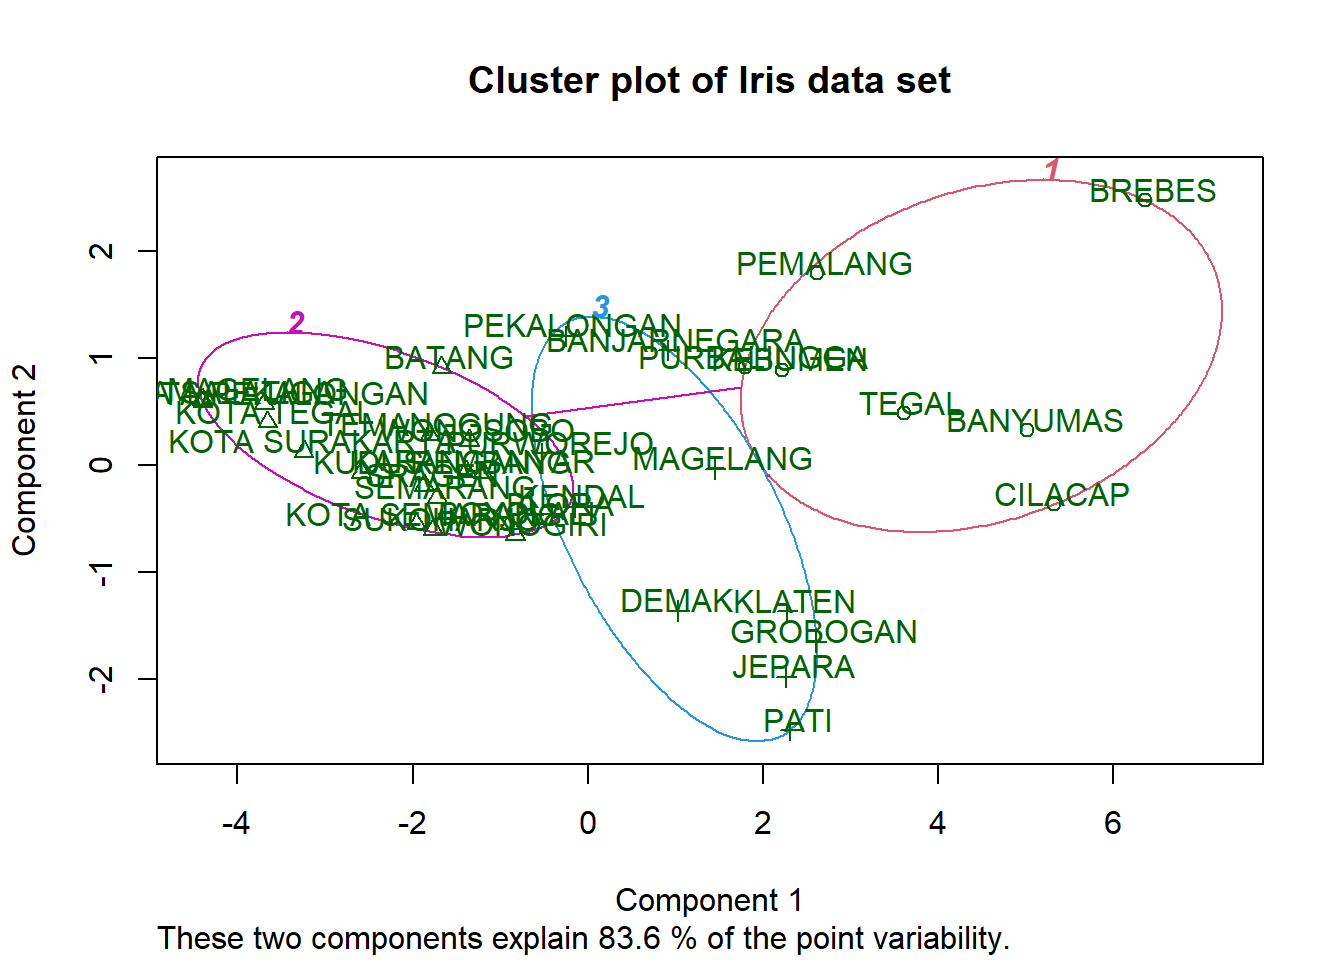
\includegraphics{03-HC_files/figure-latex/unnamed-chunk-14-1.pdf}

\begin{Shaded}
\begin{Highlighting}[]
\CommentTok{\# Compute distances and hierarchical clustering}
\NormalTok{dd }\OtherTok{\textless{}{-}} \FunctionTok{dist}\NormalTok{(}\FunctionTok{scale}\NormalTok{(data), }\AttributeTok{method =} \StringTok{"euclidean"}\NormalTok{)}
\NormalTok{hc }\OtherTok{\textless{}{-}} \FunctionTok{hclust}\NormalTok{(dd, }\AttributeTok{method =} \StringTok{"ward.D2"}\NormalTok{)}
\end{Highlighting}
\end{Shaded}

\begin{Shaded}
\begin{Highlighting}[]
\FunctionTok{library}\NormalTok{(factoextra)}
\FunctionTok{fviz\_dend}\NormalTok{(hc, }\AttributeTok{cex =} \FloatTok{0.5}\NormalTok{)}
\end{Highlighting}
\end{Shaded}

\includegraphics{03-HC_files/figure-latex/unnamed-chunk-16-1.pdf}

\begin{Shaded}
\begin{Highlighting}[]
\FunctionTok{fviz\_dend}\NormalTok{(hc, }\AttributeTok{cex =} \FloatTok{0.5}\NormalTok{,}
\AttributeTok{main =} \StringTok{"Dendrogram {-} ward.D2"}\NormalTok{,}
\AttributeTok{xlab =} \StringTok{"Objects"}\NormalTok{, }\AttributeTok{ylab =} \StringTok{"Distance"}\NormalTok{, }\AttributeTok{sub =} \StringTok{""}\NormalTok{)}
\end{Highlighting}
\end{Shaded}

\includegraphics{03-HC_files/figure-latex/unnamed-chunk-17-1.pdf}

\begin{Shaded}
\begin{Highlighting}[]
\FunctionTok{fviz\_dend}\NormalTok{(hc, }\AttributeTok{cex =} \FloatTok{0.5}\NormalTok{, }\AttributeTok{horiz =} \ConstantTok{TRUE}\NormalTok{)}
\end{Highlighting}
\end{Shaded}

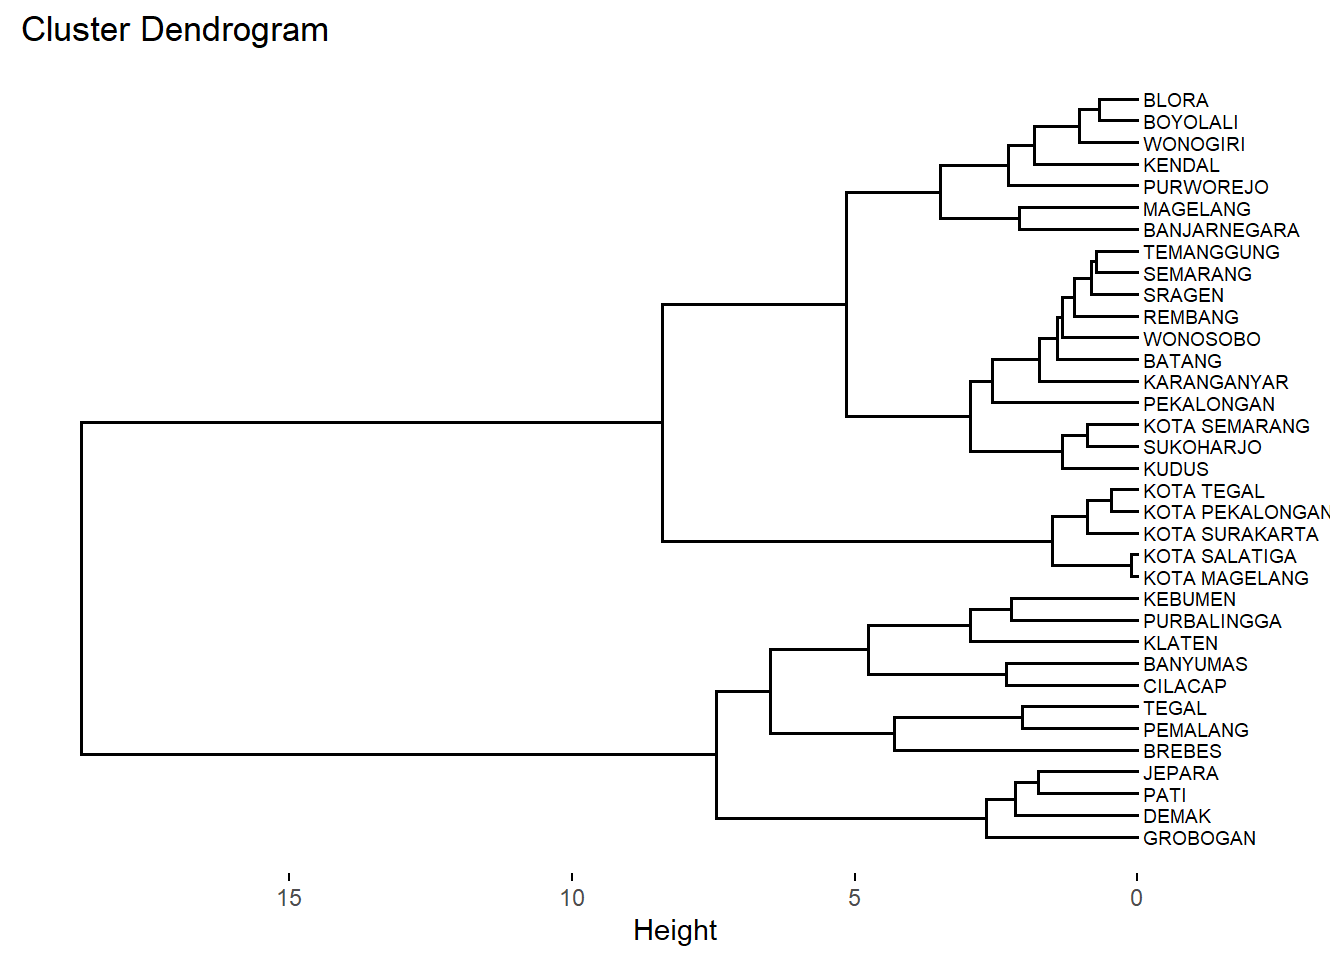
\includegraphics{03-HC_files/figure-latex/unnamed-chunk-18-1.pdf}

\begin{Shaded}
\begin{Highlighting}[]
\FunctionTok{fviz\_dend}\NormalTok{(hc, }\AttributeTok{k =}\DecValTok{2}\NormalTok{,}
\CommentTok{\# Cut in four groups}
\AttributeTok{cex =} \FloatTok{0.5}\NormalTok{,}
\CommentTok{\# label size}
\AttributeTok{k\_colors =} \FunctionTok{c}\NormalTok{(}\StringTok{"\#E7B800"}\NormalTok{, }\StringTok{"\#FC4E07"}\NormalTok{),}
\AttributeTok{color\_labels\_by\_k =} \ConstantTok{TRUE}\NormalTok{, }\CommentTok{\# color labels by groups}
\AttributeTok{ggtheme =} \FunctionTok{theme\_gray}\NormalTok{()}
\CommentTok{\# Change theme}
\NormalTok{)}
\end{Highlighting}
\end{Shaded}

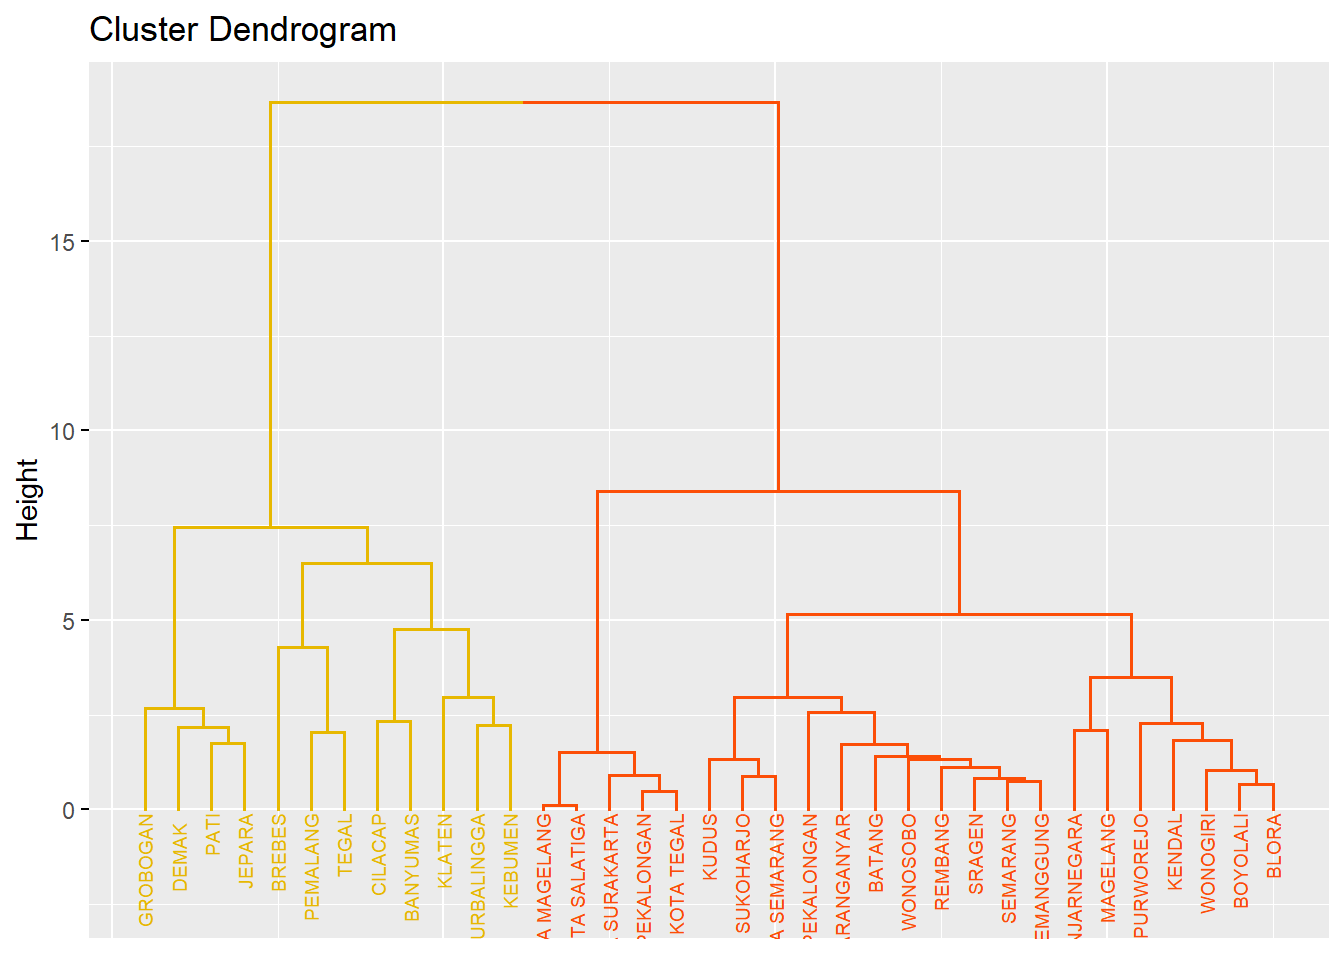
\includegraphics{03-HC_files/figure-latex/unnamed-chunk-19-1.pdf}

\begin{Shaded}
\begin{Highlighting}[]
\FunctionTok{fviz\_dend}\NormalTok{(hc, }\AttributeTok{cex =} \FloatTok{0.5}\NormalTok{, }\AttributeTok{k =}\DecValTok{2}\NormalTok{, }\CommentTok{\# Cut in four groups}
\AttributeTok{k\_colors =} \StringTok{"jco"}\NormalTok{)}
\end{Highlighting}
\end{Shaded}

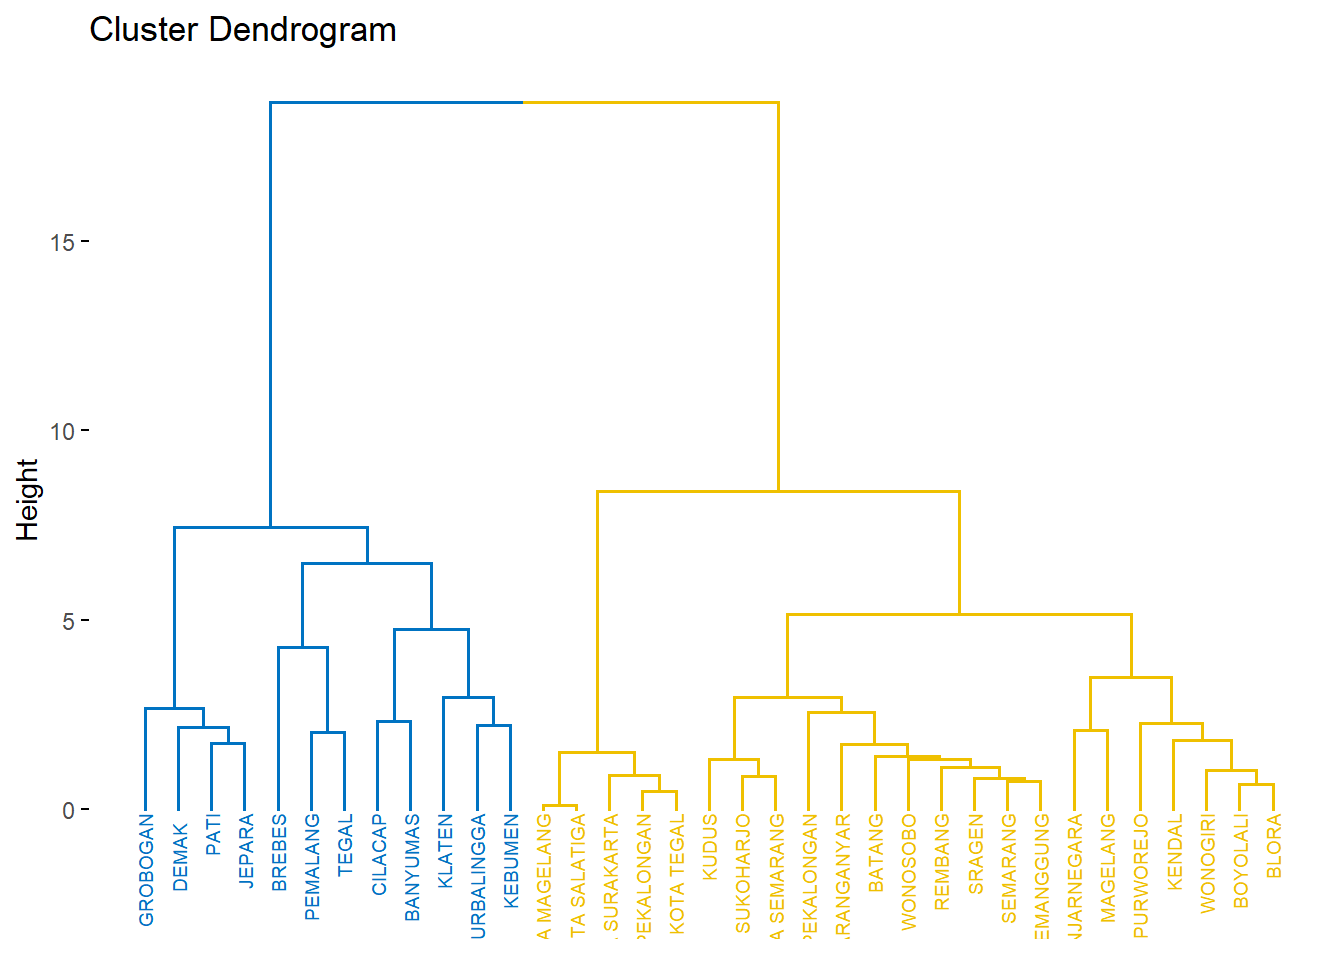
\includegraphics{03-HC_files/figure-latex/unnamed-chunk-20-1.pdf}

\begin{Shaded}
\begin{Highlighting}[]
\FunctionTok{fviz\_dend}\NormalTok{(hc, }\AttributeTok{k =}\DecValTok{2}\NormalTok{, }\AttributeTok{cex =} \FloatTok{0.4}\NormalTok{, }\AttributeTok{horiz =} \ConstantTok{TRUE}\NormalTok{, }\AttributeTok{k\_colors =} \StringTok{"jco"}\NormalTok{,}
\AttributeTok{rect =} \ConstantTok{TRUE}\NormalTok{, }\AttributeTok{rect\_border =} \StringTok{"jco"}\NormalTok{, }\AttributeTok{rect\_fill =} \ConstantTok{TRUE}\NormalTok{)}
\end{Highlighting}
\end{Shaded}

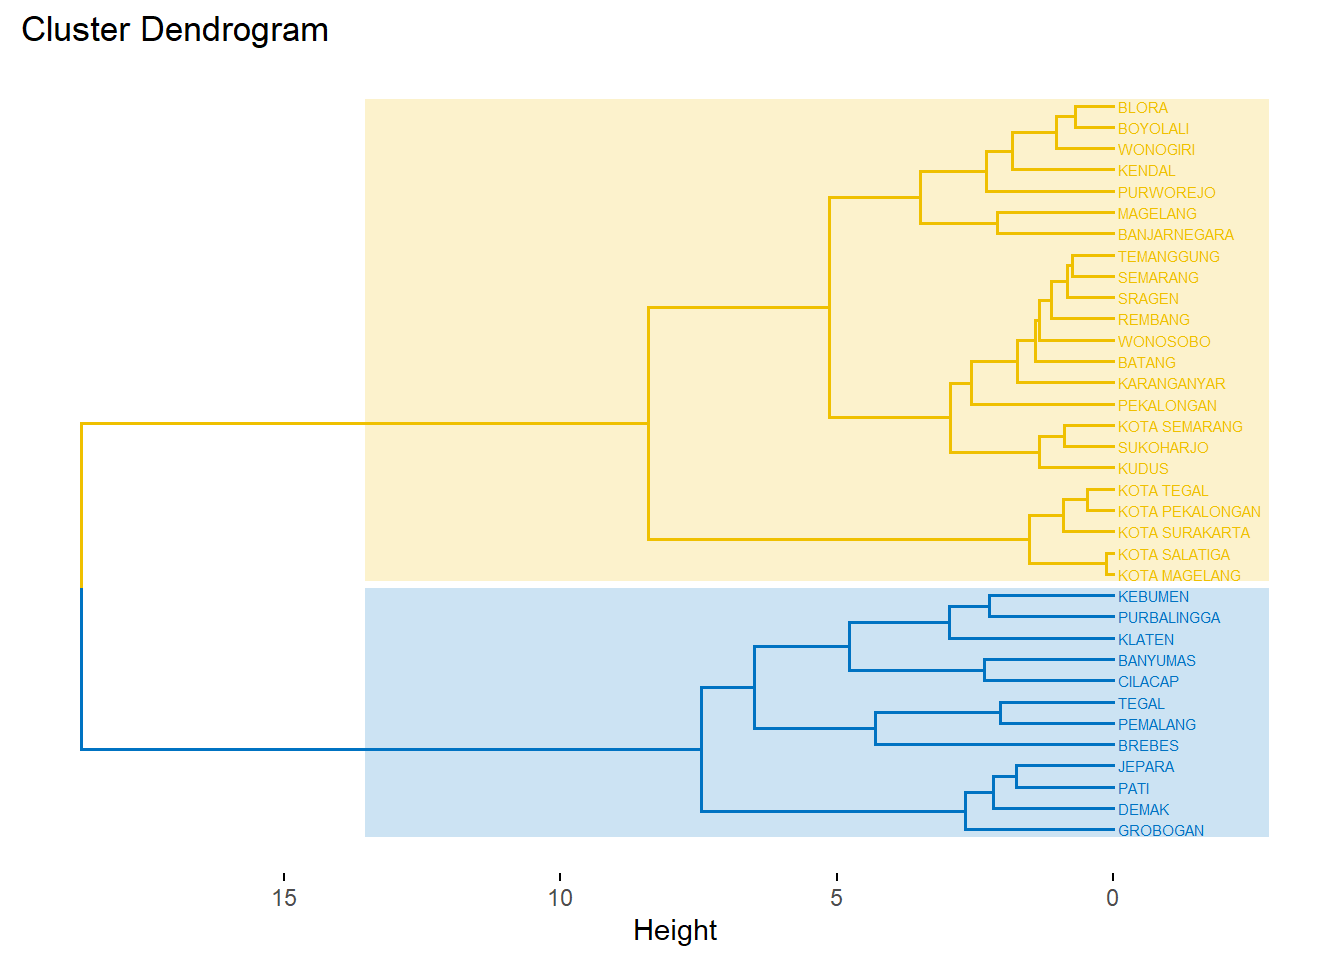
\includegraphics{03-HC_files/figure-latex/unnamed-chunk-21-1.pdf}

\begin{Shaded}
\begin{Highlighting}[]
\FunctionTok{fviz\_dend}\NormalTok{(hc, }\AttributeTok{cex =} \FloatTok{0.5}\NormalTok{, }\AttributeTok{k =}\DecValTok{2}\NormalTok{,}
\AttributeTok{k\_colors =} \StringTok{"jco"}\NormalTok{, }\AttributeTok{type =} \StringTok{"circular"}\NormalTok{)}
\end{Highlighting}
\end{Shaded}

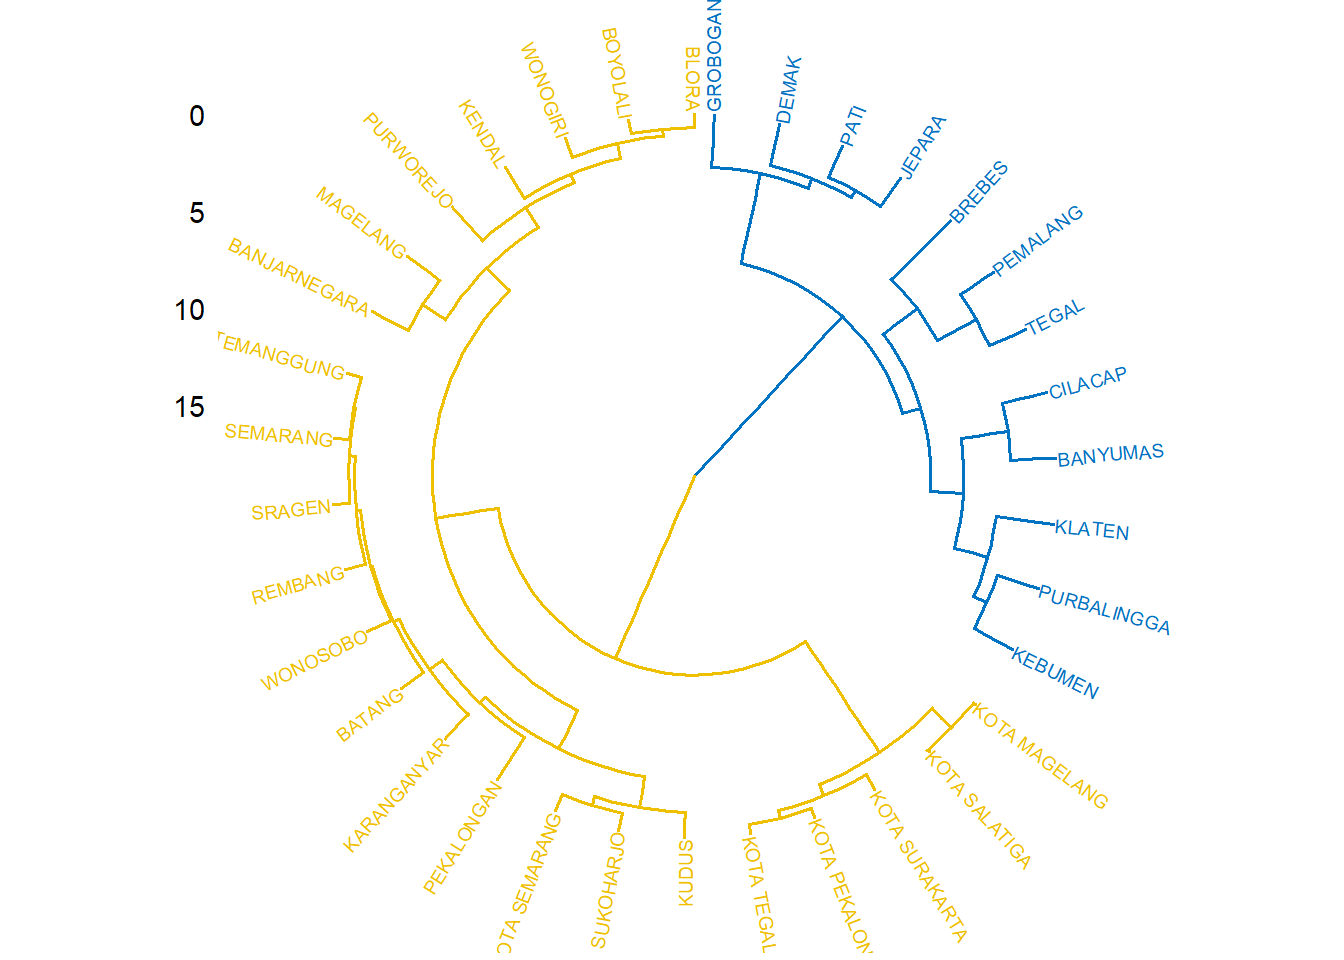
\includegraphics{03-HC_files/figure-latex/unnamed-chunk-22-1.pdf}

\begin{Shaded}
\begin{Highlighting}[]
\FunctionTok{require}\NormalTok{(}\StringTok{"igraph"}\NormalTok{)}
\end{Highlighting}
\end{Shaded}

\begin{verbatim}
## Loading required package: igraph
\end{verbatim}

\begin{verbatim}
## 
## Attaching package: 'igraph'
\end{verbatim}

\begin{verbatim}
## The following objects are masked from 'package:stats':
## 
##     decompose, spectrum
\end{verbatim}

\begin{verbatim}
## The following object is masked from 'package:base':
## 
##     union
\end{verbatim}

\begin{Shaded}
\begin{Highlighting}[]
\FunctionTok{fviz\_dend}\NormalTok{(hc, }\AttributeTok{k =}\DecValTok{2}\NormalTok{, }\AttributeTok{k\_colors =} \StringTok{"jco"}\NormalTok{,}
\AttributeTok{type =} \StringTok{"phylogenic"}\NormalTok{, }\AttributeTok{repel =} \ConstantTok{TRUE}\NormalTok{)}
\end{Highlighting}
\end{Shaded}

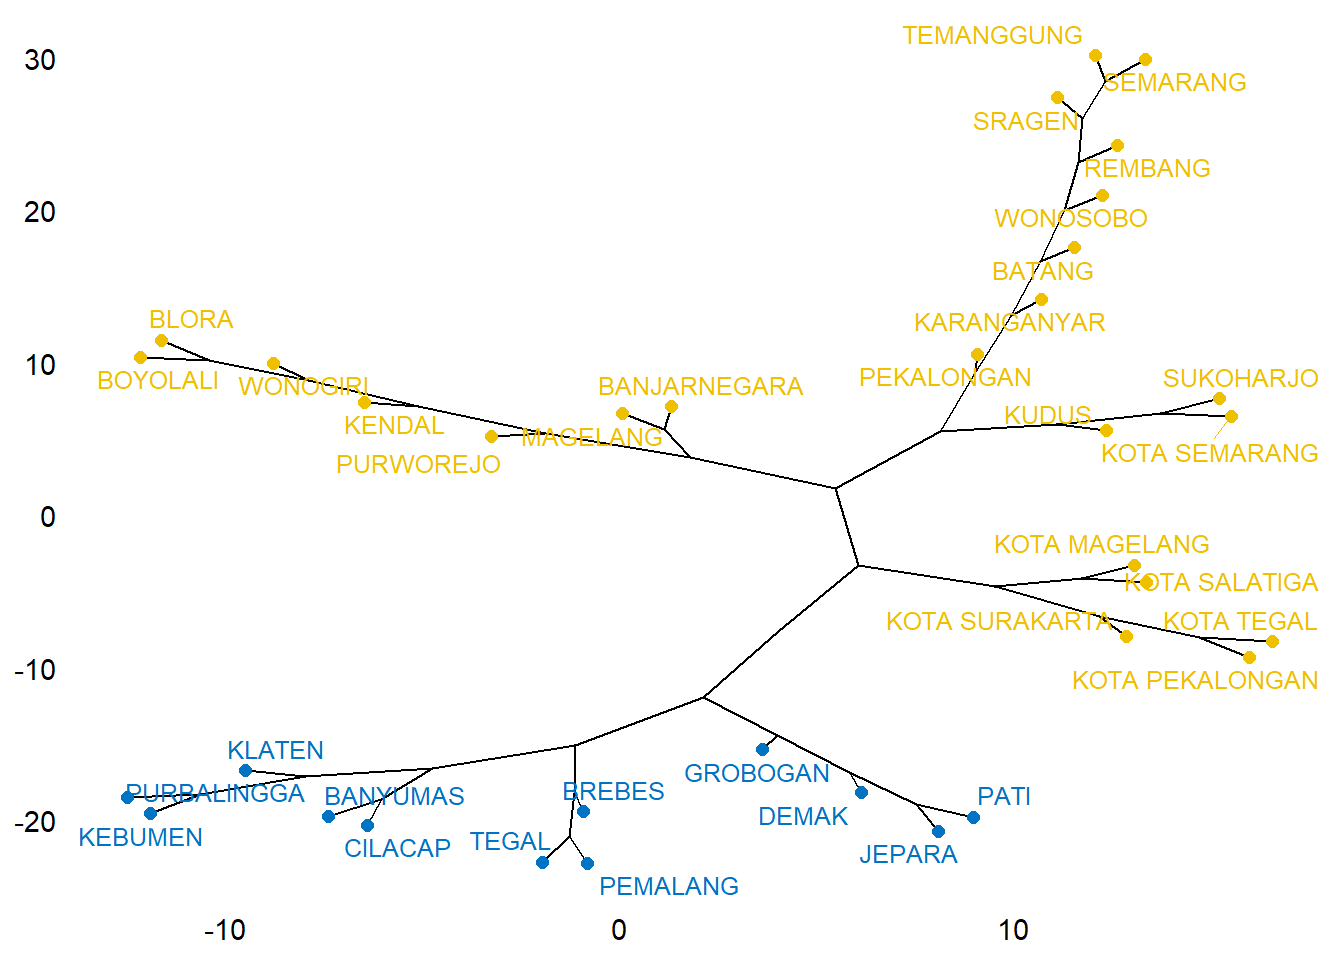
\includegraphics{03-HC_files/figure-latex/unnamed-chunk-23-1.pdf}

\begin{Shaded}
\begin{Highlighting}[]
\FunctionTok{require}\NormalTok{(}\StringTok{"igraph"}\NormalTok{)}
\FunctionTok{fviz\_dend}\NormalTok{(hc, }\AttributeTok{k =}\DecValTok{2}\NormalTok{, }\CommentTok{\# Cut in four groups}
\AttributeTok{k\_colors =} \StringTok{"jco"}\NormalTok{,}
\AttributeTok{type =} \StringTok{"phylogenic"}\NormalTok{, }\AttributeTok{repel =} \ConstantTok{TRUE}\NormalTok{,}
\AttributeTok{phylo\_layout =} \StringTok{"layout.gem"}\NormalTok{)}
\end{Highlighting}
\end{Shaded}

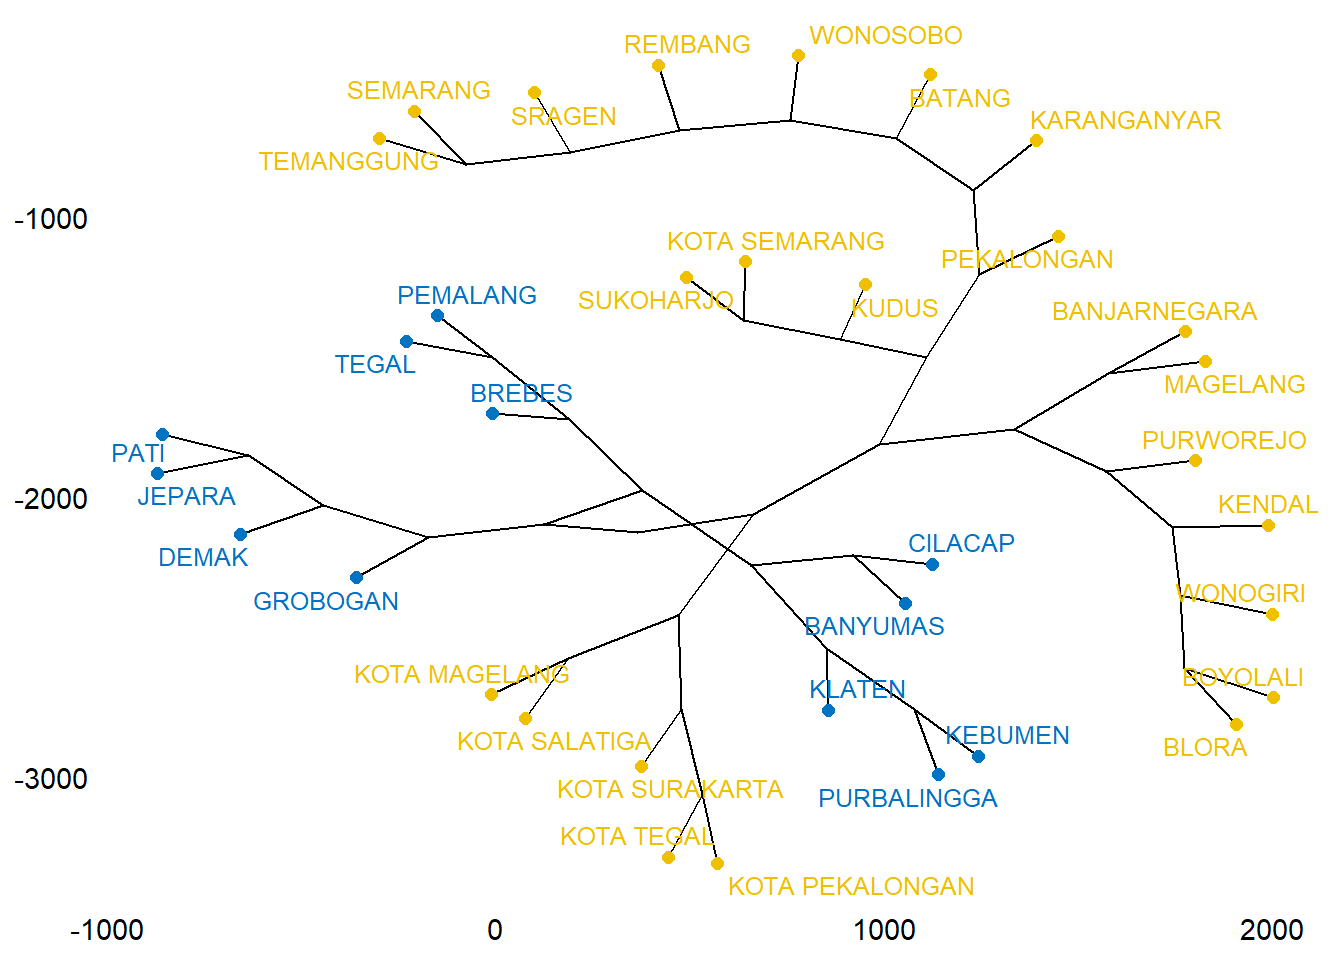
\includegraphics{03-HC_files/figure-latex/unnamed-chunk-24-1.pdf}

\hypertarget{evaluasi-analisis-cluster}{%
\chapter{Evaluasi Analisis Cluster}\label{evaluasi-analisis-cluster}}

This is an R Markdown document. Markdown is a simple formatting syntax for authoring HTML, PDF, and MS Word documents. For more details on using R Markdown see \url{http://rmarkdown.rstudio.com}.

When you click the \textbf{Knit} button a document will be generated that includes both content as well as the output of any embedded R code chunks within the document. You can embed an R code chunk like this:

\begin{Shaded}
\begin{Highlighting}[]
\FunctionTok{summary}\NormalTok{(cars)}
\end{Highlighting}
\end{Shaded}

\begin{verbatim}
##      speed           dist       
##  Min.   : 4.0   Min.   :  2.00  
##  1st Qu.:12.0   1st Qu.: 26.00  
##  Median :15.0   Median : 36.00  
##  Mean   :15.4   Mean   : 42.98  
##  3rd Qu.:19.0   3rd Qu.: 56.00  
##  Max.   :25.0   Max.   :120.00
\end{verbatim}

\hypertarget{including-plots}{%
\section{Including Plots}\label{including-plots}}

You can also embed plots, for example:

\begin{Shaded}
\begin{Highlighting}[]
\FunctionTok{par}\NormalTok{(}\AttributeTok{mar =} \FunctionTok{c}\NormalTok{(}\DecValTok{4}\NormalTok{, }\DecValTok{4}\NormalTok{, .}\DecValTok{1}\NormalTok{, .}\DecValTok{1}\NormalTok{))}
\FunctionTok{plot}\NormalTok{(pressure)}
\end{Highlighting}
\end{Shaded}

\begin{figure}

{\centering 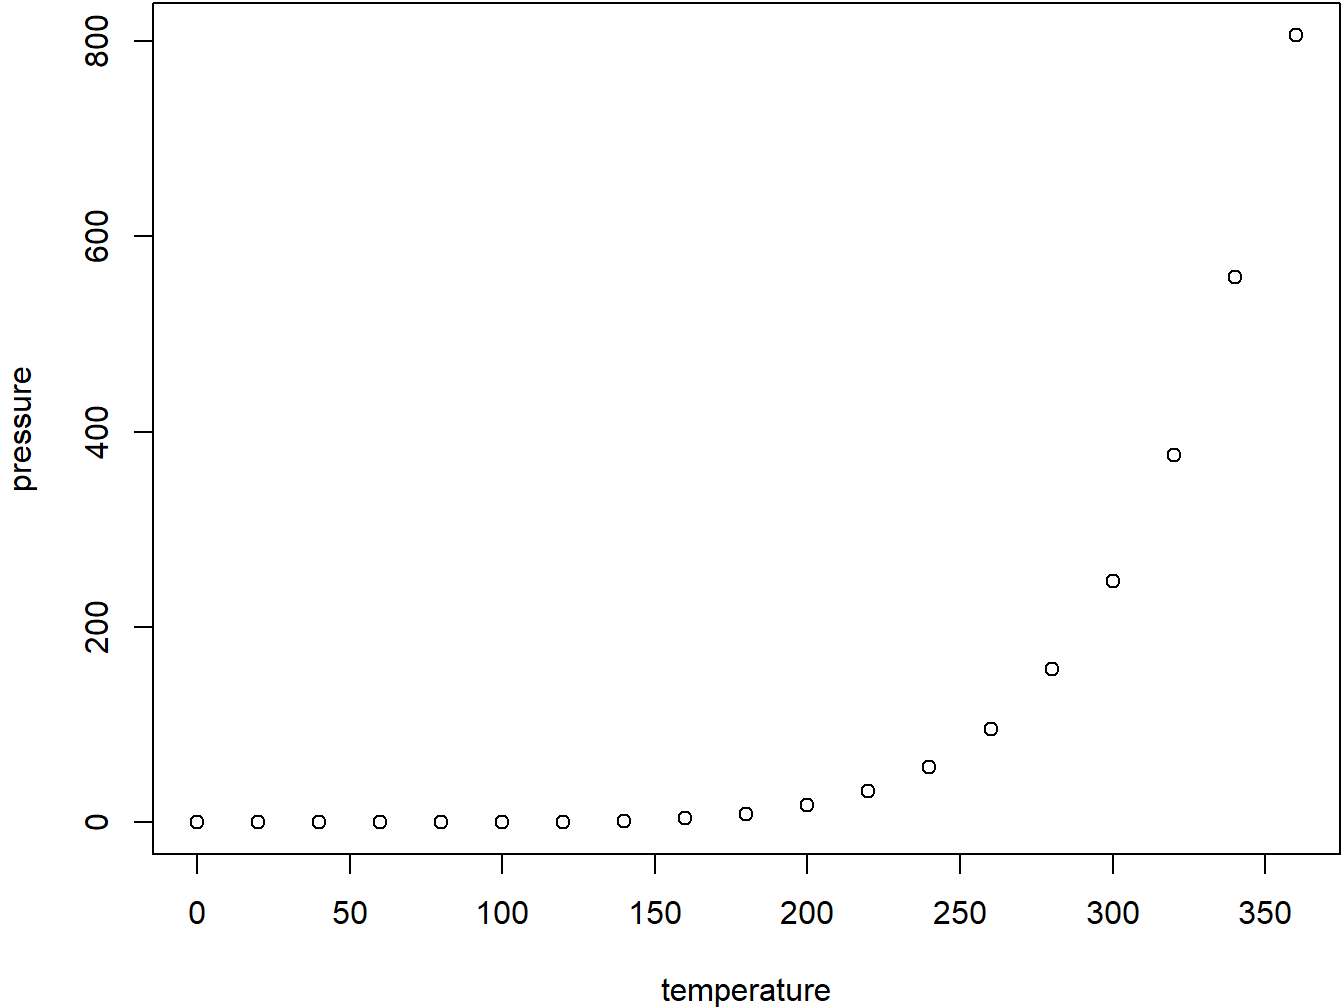
\includegraphics[width=0.8\linewidth]{19-evalC_files/figure-latex/nice-fig-02-1} 

}

\caption{Here is another nice figure!}\label{fig:nice-fig-02}
\end{figure}

Note that the \texttt{echo\ =\ FALSE} parameter was added to the code chunk to prevent printing of the R code that generated the plot.

\hypertarget{References}{%
\chapter*{Referensi}\label{References}}
\addcontentsline{toc}{chapter}{Referensi}

\hypertarget{refs}{}
\begin{CSLReferences}{1}{0}
\leavevmode\vadjust pre{\hypertarget{ref-2014clustering}{}}%
Aggarwal, Charu C., and Chandan K. Reddy, eds. 2014. \emph{Data Clustering: Algorithms and Applications}. CRC Press. \url{http://www.charuaggarwal.net/clusterbook.pdf}.

\leavevmode\vadjust pre{\hypertarget{ref-bandyopadhyay2011}{}}%
Bandyopadhyay, Sanghamitra, Sriparna Saha, and Witold Pedrycz. 2011. {``Use of a Fuzzy Granulation{\textendash}degranulation Criterion for Assessing Cluster Validity.''} \emph{Fuzzy Sets and Systems} 170 (1): 22--42. \url{https://doi.org/10.1016/j.fss.2010.11.015}.

\leavevmode\vadjust pre{\hypertarget{ref-bezdek1984}{}}%
Bezdek, James C., Robert Ehrlich, and William Full. 1984. {``FCM: The Fuzzy c-Means Clustering Algorithm.''} \emph{Computers \& Geosciences} 10 (2-3): 191--203. \url{https://doi.org/10.1016/0098-3004(84)90020-7}.

\leavevmode\vadjust pre{\hypertarget{ref-HanEtAl11}{}}%
Han, Jiawei, Micheline Kamber, and Jian Pei. 2011. \emph{Data Mining: Concepts and Techniques}. 3rd ed. San Francisco, CA, USA: Morgan Kaufmann Publishers.

\leavevmode\vadjust pre{\hypertarget{ref-pimentel2016}{}}%
Pimentel, Bruno Almeida, and Renata M. C. R. de Souza. 2016. {``Multivariate Fuzzy C-Means Algorithms with Weighting.''} \emph{Neurocomputing} 174 (January): 946--65. \url{https://doi.org/10.1016/j.neucom.2015.10.011}.

\leavevmode\vadjust pre{\hypertarget{ref-stetco2015}{}}%
Stetco, Adrian, Xiao-Jun Zeng, and John Keane. 2015. {``Fuzzy C-Means++: Fuzzy C-Means with Effective Seeding Initialization.''} \emph{Expert Systems with Applications} 42 (21): 7541--48. \url{https://doi.org/10.1016/j.eswa.2015.05.014}.

\end{CSLReferences}

\end{document}
